\documentclass[12pt,a4paper]{report}
\usepackage[italian]{babel}
\usepackage[utf8]{inputenc}
\usepackage{bold-extra}
\usepackage{graphicx}
\usepackage{listings}
\usepackage{amssymb}
\usepackage{amsmath}
\usepackage{algorithm}
\usepackage{algorithmic}
\textwidth=420pt\oddsidemargin=0pt
\newcommand{\argmax}{\mathop{\mathrm{arg\,max}}}

\begin{document}
    \pagenumbering{roman}
    \begin{titlepage}
        \begin{center}
            {{\Large{\textsc{Universit\`a degli Studi di Bari $\cdot$ Aldo Moro
            }}}} \\
            \vspace{5mm}
            
\includegraphics[width=35mm]{logouniba}\\
            \vspace{5mm}
            \Large{\textsc{Dipartimento di Informatica}} \rule[0.1cm]{15.8cm}{0.1mm}
            \rule[0.5cm]{15.8cm}{0.6mm}
            {\small{\textsc {
            \vspace{5mm}
            Corso di Laurea in Informatica}}}
        \end{center}
        \vspace{15mm}
        \begin{center}
            {\LARGE\textbf{Next-Activity Prediction tramite \break Reti Convoluzionali Deformabili}}\\
            {\LARGE{\bf --}}\\
            \vspace{15mm} {\large{\sc Tesi di Laurea in 
            \\ Algoritmi e Strutture Dati}}
        \end{center}
        \vfill
        \par
        \noindent
        \begin{minipage}[t]{0.47\textwidth}
            \vspace{10mm} {\large{\sc Relatore:}\\
            {\bf \textsc{Chiar.mo Prof.\\
             Nicola Di Mauro}}}
        \end{minipage}
        \hfill
        \begin{minipage}[t]{0.47\textwidth}\raggedleft
            \vspace{10mm} {\large{\sc Laureando:}\\
            %\vspace{2mm}
            {\bf Antonio Matteo Carulli}}
        \end{minipage}
        \begin{center}
            {\vspace{5mm} \large{\sc LACAM \\
            \vspace{10mm} Anno Accademico 2018/2019}}%inserire l'anno accademico a cui si è iscritti
        \end{center}
    \end{titlepage}
    \newpage
        \pagebreak
        \hspace{0pt}
        \vfill
        \begin{center}
            \textit{Questa pagina \`e stata intenzionalmente lasciata 
            in bianco.}
        \end{center}
        \vfill
        \hspace{0pt}
        \pagebreak
    \newpage
    \tableofcontents
    \newpage
    \pagenumbering{arabic}
    \begin{abstract}
    In una realt\`a sempre pi\`u data-driven, i sistemi informativi
    aziendali raccolgono dati sulle attivit\`a interne di 
    un'azienda, registrando eventi e processi che rappresentano 
    modelli dell'azienda stessa. Il machine learning e, pi\`u di
    recente, il deep learning sono ormai soluzioni di default per 
    l'estrazione di informazione dai dati. La disciplina del 
    Process Mining applica queste tecniche ai processi di 
    un'azienda per ottimizzarli, individuando colli di bottiglia e
    prevedendone l'andamento. I primi approcci sui dati sequenziali
    di un processo aziendale prevedevano l'uso di reti neurali 
    ricorrenti LSTM e GRU, sviluppate specificatamente per trattare
    serie temporali. Alcune recenti implementazioni, invece, hanno 
    proposto l'uso di reti convoluzionali, solitamente applicate a 
    compiti di computer vision, per ottenere risultati altrettanto 
    soddisfacenti ad un costo computazionale ridotto. In questo 
    lavoro di tesi si \`e voluto mettere a confronto una architettura 
    convoluzionale classica con un approccio convoluzionale deformabile,
    sviluppato per venire incontro ai limiti delle prime, mutuato dalla
    computer vision e adattato al compito di process mining della 
    next-activity prediction.
    \end{abstract}
    \newpage
    \chapter{Process Mining}
    \section{Cenni Storici}
    La prima citazione di processo \`e da ricercare nelle
    teorie dell'economista scozzese Adam Smith, il quale,
    nel XVIII secolo, descrisse le operazioni necessarie
    alla produzione di una spilla in diciotto passi,
    mettendo enfasi sul fatto che gli stessi, in un periodo
    caratterizzato da beni prodotti a mano, erano spesso
    effettuati dallo stesso individuo~\cite{smith1827inquiry}.
    In un suo articolo, Smith descriveva come tramite la 
    divisione organizzata del lavoro, i lavoratori della 
    fabbrica di spille potevano arrivare a produrre oltre 
    duecento volte il numero di spille normalmente realizzabili. 
    ~\cite{business-process-handbook}.
    Sebbene le idee di Smith sulla divisione del lavoro
    vennero largamente impiegate, l'integrazione dei
    compiti in un processo funzionale venne considerata
    solo nel secolo successivo con Frederick Winslow Taylor, 
    il quale nel suo Principles of Scientific Management
    si concentrava sulla standardizzazione dei processi 
    (industriali) e una chiara divisione dei ruoli sia per
    i dirigenti che per i lavoratori~\cite{principlesscimanagement}.

    \medskip
    Le prime definizioni di processo aziendale si hanno nel
    XX secolo con Davenport~\cite{davenport1993process}, che lo 
    descrive come: 
    \begin{quote}
    "...un insieme strutturato di attivit\`a progettate per
    la realizzazione di uno specifico output per soddisfare
    le richieste di uno specifico cliente o mercato"
    \end{quote}
    Definendo poi un processo aziendale come:
    \begin{quote}
    "...la struttura secondo la quale un'azienda fa ci\`o 
    che \`e necessario per realizzare un prodotto di valore
    per il cliente"
    \end{quote}

    Definizione estesa da Rummler \& Brache due anni dopo,
    con la distinzione in processi operativi, il cui output \`e
    un prodotto per il cliente, e processi di supporto, 
    il cui output \`e invisibile al cliente ma essenziale
    ai dirigenti dell'azienda~\cite{rummler1990improving}. 

    \medskip
    In accordo alla norma ISO 9001, i processi aziendali
    di aziende dotate di un sistema di gestione della
    qualit\`a devono essere misurabili e monitorabili nel
    tempo mediante l'utilizzo di indicatori di prestazione
    chiave~\cite{iso9001}.
    
    \medskip
    Definita la propria mission, un'azienda definisce i
    propri processi aziendali per raggiungere gli obiettivi
    prefissati e creare valore. 

    \section{Processo Aziendale}
    In economia aziendale il processo aziendale (business
    process) \`e un insieme di attivit\`a interrelate,
    svolte all'interno dell'azienda nell'ambito della
    gestione operativa delle sue funzioni aziendali,
    che creano valore trasformando delle risorse (input del
    processo) in un prodotto finale (output del processo) a
    valore aggiunto, destinato ad un soggetto interno o
    esterno all'azienda (cliente) e teso al raggiungimento
    di un obiettivo aziendale.

    \medskip
    Un processo aziendale quindi, descrive \textit{come} un
    prodotto o servizio deve essere realizzato, scomponendo
    l'atto di produzione in una serie di attivit\`a ben
    definite. Possiamo quindi riformulare un processo come 
    una sequenza di attivit\`a rappresentanti un'azione
    svolta da un agente, sia esso umano o macchina.
    Tipicamente, un'azione si manifesta come un'operazione
    su un oggetto fisico o informativo oppure come una 
    decisione presa da un agente coinvolto nel processo.

    \medskip
    La rappresentazione di un processo aziendale segue
    solitamente la rappresentazione a diagrammi di flusso
    dell'informatica in cui ogni azione \`e rappresentata
    come una figura geometrica collegata ad altre azioni
    o operazioni di controllo. Questo permette di avere una
    chiara definizione della sequenza di azioni da svolgere
    e di conseguenza anche delle loro dipendenze. Oltre 
    alla rappresentazione, la stessa progettazione di un 
    processo aziendale \`e spesso condivisa con i tipici
    approcci dell'informatica. In entrambe le 
    discipline infatti, un problema viene affrontato 
    scomponendo il risultato finale in operazioni 
    elementari poi riordinate per ottenere le prestazioni
    migliori con il miglior utilizzo delle risorse 
    disponibili avendo sempre a mente il risultato finale~\cite{business-process-handbook}.
    ~\cite{shankararaman2012business}.

    \section{Process Mining}
    Il termine Process Mining si riferisce all'analisi di 
    \textit{processi aziendali} tramite l'estrazione di
    conoscenza da \textit{log di eventi} ottenuti dai
    moderni sistemi informativi aziendali sfruttando 
    tecniche predittive tipiche del data mining.
    La nascita della disciplina \`e legata in parte alla
    crescita della mole di dati sugli eventi aziendali
    registrata dai sistemi informativi e in parte dal
    bisogno di supportare e migliorare i processi aziendali
    in ambienti competitivi e in rapido cambiamento.

    \subsection{Event Log}
    Fondamento del Process Mining \`e l'analisi di un
    event log, ovvero un registro ordinato di eventi
    caratterizzati da una attivit\`a associata a un
    particolare caso e un riferimento temporale, oltre ad
    eventuali altri dati a supporto. Un processo
    completato viene chiamato \textit{traccia}, possiamo
    quindi ridefinire un event log come un insieme di
    tracce in cui uno specifico evento compare al pi\`u
    una volta in tutto il registro.

    \subsubsection{Next-Activity Prediction}
    Uno dei problemi di maggiore attenzione, in quest'area
    di ricerca \`e lo sviluppo di modelli predittivi i
    quali, una volta appresi, possono essere sfruttati
    per predire tracce mancanti o l'evoluzione del processo
    in corso basandosi sui pattern estratti da un log 
    completato. La motivazione alla base del problema deriva dalla
    supposizione che analizzando processi di successo 
    gi\`a completati e mettendoli a confronto tra loro
    sia possibile generare o completare un processo in
    esecuzione di altrettanto successo. 
    Data una traccia in esecuzione, ovvero un processo
    non completato, il problema della previsione dell' attivit\`a 
    successiva consiste quindi nel prevedere la
    possibile attivit\`a seguente per la traccia corrente
    basandosi sulle informazioni estratte dal resto del 
    log~\cite{10.1007/978-3-642-28108-2_19}.

    \chapter{Apprendimento Automatico}
    \section{Intelligenza Artificiale}
    Il desiderio di creare macchine pensanti ha sfiorato spesso la
    mente dell'uomo. Le storie di Efesto, Pigmalione e Dedalo sono
    solo alcuni dei primi esempi di leggendari inventori. 
    Al giorno d'oggi, l'Intelligenza Artificiale \`e una delle 
    aree di ricerca pi\`u attive e in costante evoluzione,
    con numerose applicazioni pratiche. Agli albori della 
    disciplina, i tipi di problemi risolti dai ricercatori erano
    relativamente facili da trattare per un computer, problemi 
    descrivibili tramite regole matematiche formali, ma presto 
    affior\`o la difficolt\`a per le macchine di portare a termine 
    compiti di facile risoluzione per gli esseri umani ma difficili da 
    descrivere formalmente, il genere di compiti che eseguiamo 
    automaticamente e intuitivamente, come distinguere volti in 
    un'immagine o distinguere parole in una conversazione vocale. 
    Uno dei motivi per cui un computer ha difficolt\`a ad 
    eseguire compiti che per noi sono intuitivi deriva dal fatto che 
    questi stessi compiti sono il frutto di una vasta conoscenza sul 
    mondo applicata all'immensa mole di dati percepita ogni giorno da 
    ogni persona; per agire in maniera intelligente, un computer 
    avrebbe quindi bisogno dello stesso livello di conoscenza di
    un essere umano. L'ottenimento di questa conoscenza \`e una 
    delle principali difficolt\`a dell'Intelligenza Artificiale~\cite{Goodfellow-et-al-2016}.

    \subsubsection{Knowledge Base Systems}
    I primi approcci si basavano sulla codifica della conoscenza su
    un dato problema in un linguaggio formale che permetteva a un
    computer di effettuare ragionamenti automatici tramite regole
    logiche inferenziali. Le difficolt\`a di questo approccio, 
    chiamato \textbf{base di conoscenza}, riguardano la dipendenza
    da un team di esperti in grado di codificare efficacemente la
    propria conoscenza in regole formali adeguate~\cite{Lenat:1989:BLK:575523}.

    \section{Machine Learning} \label{mlsection}
    I limiti dei sistemi basati su basi di conoscenza hanno
    suggerito la necessit\`a di costruire sistemi intelligenti in
    grado di acquisire conoscenza autonomamente. Individuando
    pattern all'interno dei dati, un computer \`e cos\`i in grado
    di approcciare problemi che richiedono conoscenza del mondo 
    reale e prendere decisioni solitamente ritenute soggettive;
    algoritmi semplici come \textbf{naive Bayes}, infatti, possono 
    distinguere con efficacia e-mail legittime da spam. La 
    performance di questi algoritmi di machine learning dipende 
    fortemente dal modo in cui i dati di input sono rappresentati.
    Lo stesso algoritmo che distingue email di spam da email 
    legittime, ad esempio, non sarebbe in grado di ottenere le 
    \underline{stesse} informazioni estratte dal \textit{testo} del
    messaggio da una foto dello stesso, sulla falsa riga di come 
    \`e facile per gli esseri umani effettuare calcoli con il 
    sistema di numerazione arabo piuttosto che con quello romano. 
    Questo implica che per una performance ottimale \`e necessaria 
    una rappresentazione ottimale delle \textit{caratteristiche} 
    (\textbf{feature}) del problema; le difficolt\`a maggiori in 
    questo campo sono infatti la scelta delle feature e della loro
    struttura.
    
    \subsection{Representation Learning}
    A venire incontro a quest'ultimo problema \`e il 
    \textbf{representation learning} che si basa sull'apprendimento
    automatico della struttura stessa oltre che di un'associazione
    tra essa e l'output desiderato, permettendo un rapido
    adattamento del sistema a nuovi compiti minimizzando 
    l'intervento umano. Un esempio di questi sistemi sono gli
    \textit{autoencoders}, ovvero sistemi composti da due funzioni:
    un encoder, che converte l'input in una nuova rappresentazione 
    e un decoder che ritrasforma l'output precedente nella forma
    originale; gli autoencoders sono progettati per cercare di 
    mantenere quante pi\`u informazioni possibile tra le due fasi
    aggiungendo propriet\`a desiderate alle nuove rappresenazioni.
    
    \medskip
    Idealmente in questo tipo di sistemi si cerca di definire i 
    \textit{fattori di variazione} che definiscono le 
    caratteristiche dell'entit\`a di input e di decomporli per 
    ottenere i legami fondamentali tra essi e scartare le 
    informazioni superflue. Questo tipo di attivit\`a, tuttavia, 
    pu\`o essere estremamente difficile in situazioni in cui la 
    scelta della rappresentazione \`e tanto complessa quanto la 
    risoluzione del compito per un umano, come ad esempio per il 
    riconoscimento dell'accento da una registrazione.
    
    \newpage
    \subsection{Struttura di un Algoritmo di Machine Learning}
    Quasi tutti gli algoritmi di deep learning possono essere 
    descritti dai seguenti quattro elementi:
    \begin{itemize}
    \item[-] la specifica di un dataset,
    \item[-] una funzione costo,
    \item[-] una procedura di ottimizzazione,
    \item[-] un modello
    \end{itemize}
    
    \subsubsection{Dataset}
    Un compito di machine learning \`e generalmente descritto in 
    termini di \textit{come} il sistema dovrebbe elaborare un 
    \textbf{esempio}, ovvero un insieme di \textbf{features} 
    ottenute dalla misurazione di un oggetto o evento e formalmente
    definito come un vettore $\textbf{x} \in \mathbb{R}^n$ dove 
    ogni $x_i$ del vettore \`e una feature, o caratteristica. Un 
    insieme di esempi forma un \textbf{dataset}.
    
    \medskip
    La forma del dataset cambia a seconda del tipo di algoritmo di 
    apprendimento utilizzato le cui due grandi categorie principali
    sono: apprendimento supervisionato e apprendimento non 
    supervisionato. Negli \textbf{algoritmi di apprendimento 
    supervisionato} il dataset \`e composto da esempi ai quali 
    sono associati un'etichetta o un valore obiettivo, mentre negli
    \textbf{algoritmi di apprendimento non supervisionato} il 
    dataset contiene solo gli esempi. Gli approcci supervised si 
    basano quindi sull'osservazione di diversi esempi da un vettore
    casuale $\textbf{x}$ e da un valore o vettore di valori 
    associati $\textbf{y}$ e da queste osservazioni imparare a
    predire $\textbf{y}$ da $\textbf{x}$. Gli approcci 
    unsupervised, invece, si basano sull'osservazione di esempi 
    da un vettore casuale $\textbf{x}$ del quale si cerca, 
    implicitamente o esplicitamente, di derivare l'intera 
    distribuzione di probabilit\`a $p(\textbf{x})$ o altre 
    propriet\`a desiderate. Un modo comune di rappresentare un 
    dataset \`e tramite una \textbf{design matrix} che consiste in 
    una matrice le cui righe sono gli esempi e le colonne le 
    feature che compongono ogni esempio; per esempio, se avessimo 
    un dataset di 150 esempi formati da 4 features ciascuno, la 
    design matrix risultante sarebbe la matrice 
    $\textbf{\textit{X}}\in\mathbb{R}^{150x4}$.
    
    \medskip
    In fase di valutazione, si \`e interessati a quanto l'algoritmo
    \`e performante su dati che non ha mai trattato, ovvero
    la sua capacit\`a di \textbf{generalizzazione}, essendo questa 
    una diretta indicazione di come si comporter\`a con dati reali. 
    Pertanto, si misura la performance di un algoritmo su un 
    \textbf{test set} separato da quello su cui \`e stato addestrato il 
    sistema, andando a definire le matrici $\textbf{\textit{X}}^{(train)}$
    e $\textbf{\textit{X}}^{(test)}$. Nella maggior parte degli
    algoritmi di machine learning sono presenti degli iper-parametri,
    indicatori che controllano il comportamento dell'apprendimento i
    cui valori non sono adattati dall'algoritmo in s\`e, a volte 
    perch\`e troppo difficili da ottimizzare, altre perch\`e non sono il
    tipo di parametri adatti da apprendere sul training set. Pertanto,
    \`e necessario avere un \textbf{validation set} ignorato 
    dall'algoritmo di apprendimento e utilizzato per adattare gli 
    iper-parametri e stimare l'errore di generalizzazione. Non volendo 
    influenzare la scelta di nessun parametro, compresi gli 
    iper-parametri, dal test set, l'insieme di validazione viene 
    costruito da quello di training, tipicamente usandone l'80\% per il
    training e il 20\% per la validazione.
    
    \medskip
    In problemi di classificazione, una metrica comune \`e
    l'\textbf{accuracy} che consiste nella proporzione di esempi per i
    quali il modello ha generato l'output corretto. Analogamente si
    pu\`o misurare il \textbf{tasso d'errore} tramite la \textbf{loss 
    0-1} che restituisce 0 in caso di classificazione corretta e 1 
    altrimenti. Un'altra alternativa consiste invece nel calcolare l'
    \textbf{Errore Quadratico Medio}, o MSE, dall'inglese Mean Squared 
    Error, del modello sul test set. Se $\textbf{\^y}^{(test)}$ \`e il 
    vettore delle classificazioni sul test set, l'errore quadratico 
    medio \`e dato da
    \begin{equation}
      MSE_{test}=\frac{1}{m}\sum_{i}{(\hat{y}^{(test)}-y^{(test)})}^2_i,
    \end{equation}
    dove \textit{m} \`e il numero di esempi nell'input. Si nota che
    l'errore si annulla quando $\hat{y}^{(test)}=y^{(test)}$ e
    \begin{equation}
      MSE_{test}=\frac{1}{m} \| \hat{y}^{(test)}-y^{(test)} \|^2_2,
    \end{equation}
    cio\`e l'errore \`e lineare rispetto alla distanza Euclidea tra le 
    predizioni e gli obiettivi.
    
    \subsubsection{Funzione Costo e Ottimizzazione} \label{optsection}
    La funzione costo, o funzione loss o errore, rappresenta formalmente
    il modo di apprendere del sistema e varia in base al tipo di task da
    risolvere. Generalmente, la funzione costo \`e una funzione 
    parametrica derivabile lineare o non lineare. Sviluppare un 
    algoritmo di machine learning vuol dire quindi progettare un 
    algoritmo che individui i valori ottimali dei parametri, o pesi 
    (weights), $\boldsymbol{w}$ della funzione costo in maniera da 
    ridurre l'errore di generalizzazione del modello tramite 
    l'osservazione di un training set ($\boldsymbol{X}^{(train)}, 
    \boldsymbol{y}^{(train)}$). Un modo per farlo \`e quello di 
    minimizzare l'errore sul training set, ad esempio, ponendo la sua 
    derivata a 0. Avendo a che fare con funzioni parametriche e 
    tipicamente scalari che si basano su pi\`u input, \`e necessario 
    utilizzare delle derivate parziali per ogni parametro della 
    funzione; il \textbf{gradiente} di una funzione generalizza questo 
    concetto. Data una funzione $f: \mathbb{R}^n\rightarrow\mathbb{R}$,
    il suo gradiente \`e $\nabla f: \mathbb{R}^n\rightarrow\mathbb{R}^n$
    dove 
    \begin{equation}
        \nabla_{\boldsymbol{x}}f(x)=\begin{bmatrix}
        \frac{\partial f}{\partial x_1} \\
        \vdots \\
        \frac{\partial f}{\partial x_n}
    \end{bmatrix}.
    \end{equation}
    Geometricamente, la derivata di una funzione rappresenta 
    l'inclinazione della curva del grafico della funzione. In questo 
    modo, \`e possibile sfruttare il gradiente, e quindi la derivata, di
    una funzione parametrica come guida nella ricerca dei parametri che
    la riducono il pi\`u velocemente possibile. Questo \`e conosciuto 
    come il \textbf{metodo della Discesa del Gradiente} 
    ~\cite{gradientdescent} (MDG), tramite il quale si individua, 
    iterativamente, il nuovo punto
    \begin{equation}
        \textbf{x'}=\textbf{x}-\epsilon\nabla_\textbf{x}f(\textbf{x})
    \end{equation}
    dove $\epsilon$ \`e detto \textit{tasso d'apprendimento} o 
    \textbf{learning rate}: uno scalare positivo che determina la 
    grandezza dello step verso il nuovo punto. La complessit\`a legata
    al calcolo dello step successivo tende facilmente ad essere $O(m)$
    con \textit{m} numero di esempi e per dataset molto grandi, questo 
    pu\`o comportare tempi di calcolo estremamente lunghi, pertanto,
    considerando che il gradiente nel MDG non \`e altro che una 
    aspettativa, esso \`e approssimabile su un sottoinsieme di esempi.
    Questa estensione del MGD, chiamata \textbf{Discesa Stocastica del 
    Gradiente}, si basa sull'utilizzare, a ogni step del metodo, una
    \textbf{minibatch}, un piccolo sottoinsieme, di esempi $\mathbb{B}=
    \{\textbf{x}^{(1)}, \dots, \textbf{x}^{(m')}\}$ estratti uniformemente
    dall'insieme di training. La dimensione della minibatch, $m'$
    \`e genericamente scelta come valore molto basso, da uno a poche 
    centinaia, e rimane fissa al crescere della dimensione $m$ 
    del set di training.
    
    \subsubsection{Modello} \label{sec:crossval}
    Oltre a ridurre l'errore sul training set, tuttavia, si \`e 
    interessati anche a ridurre l'errore sul test set, o \textbf{errore
    di generalizzazione}; ma essendo i dati osservati dall'algoritmo 
    esclusivamente quelli del dataset di addestramento, \`e necessario
    fare delle assunzioni sui dati. I dataset di training e test sono
    generati dalla stessa distribuzione di probabilit\`a e da datasets
    comuni chiamata \textbf{processo di generazione dei dati}. Questo
    processo si basa sull'assunzione che gli esempi di ogni dataset 
    siano \textbf{indipendenti} tra loro e che training e test set siano
    \textbf{identicamente distribuiti} dalla stessa 
    \textbf{distribuzione di generazione dei dati} $p_{data}$,
    permettendo lo studio delle relazioni matematiche tra gli errori di
    training e di test. Tenendo in considerazione i parametri \textbf{w}, 
    si nota come sia necessario sceglierli dopo aver generato il
    dataset di training, basandosi sui suoi valori, e solo per ultimo
    generare il test set; se cos\`i non fosse infatti, si avrebbe un 
    errore di training identico all'errore di generalizzazione. Cos\`i
    facendo l'errore di test che si aspetta di avere \`e \textit{uguale
    o maggiore} di quello in fase di addestramento. Questo procedimento
    prende il nome di \textbf{cross validation}. I fattori che
    influenzano quanto bene un algoritmo di machine learning sar\`a in
    grado di performare, quindi, dipendono dalla sua capacit\`a di 
    minimizzare l'errore d'addestramento e la sua differenza con quello
    di test. Quando un modello non \`e in grado di ottenere un errore
    di training sufficientemente basso si ha \textbf{underfitting}, se
    il modello produce una differenza tra errore di training ed errore
    di generalizzazione troppo alta, invece, si ha \textbf{overfitting}.
    \`E possibile controllare il \textit{fitting} di un modello variando
    la sua \textbf{capacit\`a}, ovvero la sua abilit\`a di assumere la
    forma di una vasta gamma di funzioni. Una bassa capacit\`a pu\`o
    portare all'underfitting, mentre un modello con un'alta capacit\`a 
    potrebbe memorizzare propriet\`a superflue dagli esempi che 
    influiscono negativamente sull'errore in fase di test. Un modo di 
    controllare la capacit\`a di un modello \`e quello di scegliere il suo
    \textbf{spazio delle ipotesi}, ovvero l'insieme delle funzioni che
    l'algoritmo pu\`o scegliere come soluzioni. In generale, modelli
    con un'alta capacit\`a riescono a risolvere compiti anche molto
    complessi, irrisolvibili da modelli con una bassa capacit\`a, ma 
    rischiano l'overfitting se applicati a problemi pi\`u semplici.
    
    \subsection{Regularization}  \label{sec:regularization}
    Il teorema \textit{No Free Lunch} per il machine learning 
    ~\cite{Rumelhart1986} sostiene che, mediando su ogni 
    possibile distribuzione di generazione di dati, qualsiasi algoritmo
    di classificazione ottiene lo stesso tasso d'errore di fronte a dati
    che non ha mai trattato. Ci\`o che implica questo teorema \`e che
    non pu\`o esistere un algoritmo universalmente migliore degli altri.
    Tuttavia, ci\`o si applica solo nel caso in cui si abbia a che fare
    con \textit{ogni} possibile distribuzione di generazione dei dati;
    pertanto, l'approccio utilizzato \`e quello di fare di volta in 
    volta delle assunzioni circa il tipo di distribuzioni che riguardano
    uno specifico compito di machine learning, introducendo delle
    opportune \textit{preferenze} nell'algoritmo di apprendimento.
    Esistono diversi modi di esprimere queste preferenze, sia 
    implicitamente che esplicitamente. Nel collettivo, l'applicazione 
    di questi approcci \`e detta \textbf{regolarizzazione}, ovvero ogni
    modifica fatta ad un algoritmo atta a ridurre il suo errore di 
    generalizzazione lasciando invariato il suo errore di training.

    Una delle forme pi\`u comuni di regolarizzazione \`e quella dell'
    \textbf{early stopping}. Quando si addestrano modelli con una
    capacit\`a di rappresentazione sufficiente a raggiungere 
    l'overfitting si osserva spesso come l'errore di training tenda
    a diminuire costantemente nel tempo, al contrario dell'errore di
    validazione. L'approccio di early stopping si basa sull'assunzione
    che salvare i parametri ottenuti al momento in cui l'errore di 
    validazione \`e pi\`u basso permetta di ottenere un modello 
    migliore. Ogni volta che l'errore di validazione migliora, viene
    salvata una copia dei parametri associati se questa \`e maggiore
    delle precedenti. L'algoritmo termina quando non si registrano
    miglioramenti aggiuntivi nell'errore di validazione dopo un 
    prefissato numero di iterazioni.
    
    \newpage
    \subsection{Principio di Massima Verosimiglianza} \label{mllsection}
    Statisticamente la funzione costo deve essere una buona stima della
    reale distribuzione di probabilit\`a degli esempi nel dataset di 
    training. Per scegliere una buona funzione costo si utilizza 
    comunemente il \textbf{principio della massima verosimiglianza}.
    
    Dato $\mathbb{X}=\{\textbf{x}^{(1)}, \dots, \textbf{x}^{(m)}\}$ un 
    set di \textit{m} esempi scelti indipendentemente dalla ditribuzione
    di generazione di dati sconosciuta $p_{data}(\textbf{x})$. Sia 
    $p_{model}(\textbf{x};\mbox{\boldmath{$\theta$}})$ una famiglia 
    parametrica di distribuzioni di probabilit\`a sullo stesso spazio 
    identificato da $\theta$ tale che 
    $p_{model}(\textbf{x};\mbox{\boldmath{$\theta$}})$ associ a ogni
    configurazione \textbf{x} un numero reale che stima la probabilit\`a
    $p_{data}(\textbf{x})$. La stima di massima verosimiglianza per 
    $\mbox{\boldmath{$\theta$}}$ \`e
    \begin{align}
        \boldsymbol{\theta}_{MV} &= \argmax_{\boldsymbol{\theta}} p_{model}(\mathbb{X}; \boldsymbol{\theta}), \\ 
        &= \argmax_{\boldsymbol{\theta}} \prod\limits_{i=1}^m p_{model}(\textbf{x}^{(i)}; \boldsymbol{\theta}).
    \end{align}
    Si nota che il logaritmo della verosimiglianza lascia il suo argmax
    invariato ma trasforma il prodotto in una somma
    \begin{equation}
        \mbox{\boldmath{$\theta$}}_{MV} = \argmax_{\mbox{\boldmath{$\theta$}}}\sum\limits_{i=1}^mlog\ p_{model}(\textbf{x}^{(i)};{\mbox{\boldmath{$\theta$}}})
    \end{equation}
    Dividendo per $m$, lasciando invariato l'argmax, possiamo ottenere 
    una versione della funzione costo come stima della distribuzione 
    empirica $\hat{p}_{data}$ definita dai dati di training
    \begin{equation}
        \mbox{\boldmath{$\theta$}}_{MV} = \mathbb{E}_{\textbf{x}\sim\hat{p}_{data}}log\ p_{model}(\textbf{x};{\mbox{\boldmath{$\theta$}}})
    \end{equation}
    
    Un modo di interpretare la stima di massima verosimiglianza \`e 
    quello di vederla come il minimizzare la differenza tra la 
    distribuzione empirica $\hat{p}_{data}$, definita sul training set,
    e quella del modello $p_{model}$, calcolando la differenza tra le 
    due distribuzioni tramite la \textbf{divergenza di Kullback-Leibler}
    (KL) data da
    \begin{equation}
        D_{KL}(\hat{p}_{data}\ ||\ p_{model}) = \mathbb{E}_{\textbf{x}\sim\hat{p}_{data}}[log\ \hat{p}_{data}(\textbf{x})-log\ p_{model}(\textbf{x})]
    \end{equation}
    Il termine a sinistra \`e una funzione della sola distribuzione, non
    del modello, quindi quando quest'ultimo viene addestrato per
    minimizzare la divergenza KL, sar\`a sufficiente minimizzare
    \begin{equation}
        -\mathbb{E}_{\textbf{x}\sim\hat{p}_{data}}\ [log\ p_{model}(\textbf{x})]
    \end{equation}
    che equivale a minimizzare l'\textbf{entropia incrociata} tra le due
    distribuzioni, dove per entropia incrociata si intende qualsiasi 
    funzione di loss formata da una verosimiglianza logaritmica negativa
    tra la distribuzione empirica estratta dal training set e la 
    distribuzione del modello. L'errore quadratico medio, ad esempio,
    \`e l'entropia incrociata tra la distribuzione empirica e un modello
    Gaussiano.
    
    \section{Deep Learning}
    Gli approcci di \textbf{deep learning} vengono incontro ai limiti
    del representation learning scomponendo la rappresentazione
    finale in una serie di altre rappresentazioni meno complesse 
    apprese in modo progressivo dai dati di input. Uno degli esempi 
    pi\`u caratteristici \`e quello del \textbf{multi-layer perceptron} 
    (MLP).
    
    \subsection{Multi-Layer Perceptron} \label{sec:mlp}
    Un Multi-Layer Perceptron, o Feedforward Neural Network, \`e un
    tipo di rete neurale in cui si cerca di ottimizzare la funzione
    composta $f(\textbf{x}, \theta)$ che approssima una funzione 
    obiettivo $f^*(\textbf{x})$ tramite l'apprendimento dei 
    parametri $\theta$ di $f$. 
    
    Il termine \textit{feedforward} deriva dal fatto che la 
    funzione composta \`e tipicamente della forma 
    $f^*(\textbf{x})=f^{(1)}(f^{(2)}(f^{(3)}(f^{(\dots)}(\textbf{x}))))$ 
    dove ogni funzione intermedia $f^{(i)}$, detta \textit{layer}, ha 
    come input l'output del layer precedente senza essere parametro dei
    successivi, cio\`e senza avere connessioni di ritorno 
    (feedback) nella catena di funzioni cos\`i creata. L'aggettivo 
    \textit{deep} in Deep Learning deriva dalla lunghezza della 
    catena di funzioni che compongono la funzione da ottimizzare.
    Il modello assume quindi la forma di un grafo direzionato
    aciclico che rappresenta \textit{come} i vari layer interagiscono.
    All'ultimo layer, detto di \textit{output}, vengono associati 
    gli esempi di addestramento, ad esempio etichette nel caso di un 
    problema di classificazione, mentre il resto dei layer, detti 
    nascosti (\textit{hidden}), non sono direttamente influenzati dagli
    esempi.
    
    \subsection{Funzioni d'attivazione} \label{sec:activation}
    La funzione che produce l'output di ogni hidden layer deve 
    necessariamente essere non lineare; uno degli approcci pi\`u 
    comuni \`e quello di applicare delle trasformazioni affini all'input
    controllate da parametri appresi seguite poi da una funzione non 
    lineare fissa, detta di \textit{attivazione} (activation function).
    La pi\`u diffusa tra le funzioni d'attivazione \`e la
    \textit{Rectified Linear Unit}, o \textbf{ReLU}, definita come:
    \begin{equation}
        g(z) = max(0, z)
    \end{equation}
    La non linearit\`a di queste funzioni porta la funzione costo ad 
    essere non convessa. Per funzioni convesse, il processo di 
    ottimizzazione converge a partire da qualsiasi parametro iniziale,
    ma per funzioni non convesse il metodo della discesa stocastica del
    gradiente \`e sensibile a questi e non garantisce sempre la 
    convergenza; per questo motivo, si preferisce inizializzare i pesi 
    delle reti neurali a valori casuali molto bassi.
    La maggior parte delle volte, si utilizza l'entropia incrociata tra
    la distribuzione dei dati e quella del modello come funzione costo
    determinandone la forma in base al modo di rappresentare l'output.
    Supponendo che la rete neurale produca un set di features nascoste
    $\textbf{h}=f(\textbf{x}, \mbox{\boldmath{$\theta$}})$ infatti, il
    ruolo dell'unit\`a di output \`e quello di effettuare le ultime 
    trasformazioni sulla base delle feature $\textbf{h}$ per completare
    il compito che la rete deve svolgere.
    
    \subsection{Unit\`a lineari}
    Un'unit\`a basata su trasformazioni affini senza nonlinearit\`a 
    viene comunemente chiamata unit\`a lineare. Date le features 
    $\boldsymbol{h}$ un layer di unit\`a lineari produce il vettore
    $\boldsymbol{\hat{y}}=\boldsymbol{W}^\intercal\ \boldsymbol{h}+\boldsymbol{b}$.
    Tipicamente, questo tipo di layer sono usati per produrre la media
    di una distribuzione Gaussiana condizionale
    \begin{equation}
        p(\boldsymbol{y}\ |\ \boldsymbol{x})=\mathcal{N}(\boldsymbol{y};\boldsymbol{\hat{y}},\boldsymbol{I})
    \end{equation}
    per la quale massimizzare la verosimiglianza logaritmica equivale 
    a minimizzare l'errore quadratico medio. Gli algoritmi di 
    ottimizzazione basati sul gradiente non incontrano difficolt\`a con
    questo tipo di layer in quanto non saturano, cio\`e non incontrano 
    mai asintoti orizzontali.
    
    \subsection{Funzione Softmax} \label{sec:softmax}
    Volendo rappresentare una distribuzione di probabilit\`a su una 
    variabile discreta con $n$ possibili valori, come nel caso di un 
    problema di classificazione a pi\`u classi, si pu\`o utilizzare la 
    funzione \textbf{softmax}. Innanzitutto, si vuole generare un 
    vettore di probabilit\`a $\mbox{\boldmath{$\hat{y}$}}$ con 
    $\hat{y}_i= P(y=i|\textbf{x})$. Per ottenere una distribuzione 
    valida, ogni $\hat{y}_i$ deve essere compreso tra 0 e 1 e la somma 
    dell'intero vettore deve essere 1. Per assicurarsi di avere sempre
    valori che generano un buon gradiente, applichiamo un layer lineare
    prima della funzione d'attivazione. L'unit\`a lineare predice le
    probabilit\`a logaritmiche non normalizzate
    \begin{equation}
        \boldsymbol{z}=\boldsymbol{W}^\intercal\ \boldsymbol{h}+\boldsymbol{b}
    \end{equation}
    dove $z_i=log\ \hat{P}(y=i\ |\ \boldsymbol{x})$. La funzione softmax esegue 
    l'esponenziale e normalizza i valori per ottenere la $\mbox{\boldmath{$\hat{y}$}}$ 
    desiderata. Formalmente
    \begin{equation}
        \mathrm{softmax}(\boldsymbol{z})_i = \frac{\exp(z_i)}{\sum\limits_{j}\exp(z_j)}
    \end{equation}
    La presenza dell'esponenziale permette alla funzione softmax di 
    interagire bene con il metodo della massima verosimiglianza 
    logaritmica. In questo caso, si vuole massimizzare $\log\ P(y=i|
    \boldsymbol{x})=\log\mathrm{softmax}(\boldsymbol{z})_i$, quindi \`e
    naturale esprimere la softmax in termini dell'esponenziale dato che
    questo si semplifica con il logaritmo della massima verosimiglianza
    \begin{equation} \label{logsoftmax}
       \log\mathrm{softmax}(\boldsymbol{z})_i=z_i-\log\sum\limits_j\exp(z_j)
    \end{equation}
    Si nota come nel primo termine dell'equazione \ref{logsoftmax}, 
    l'input $z_i$ ha sempre un contributo diretto nella funzione costo,
    ma ci\`o non intacca il processo d'apprendimento in quanto la 
    variabile $\boldsymbol{z}$, detta \textbf{logit}, non pu\`o saturare
    e nemmeno nel caso in cui il secondo termine, che porta l'intero 
    vettore $\boldsymbol{z}$ a diminuire, \`e molto piccolo. 
    Analizzando ulteriormente il secondo termine 
    $\log\sum_j\exp(z_j)$ si fa notare come esso pu\`o essere
    approssimato a $\max_jz_j$ dato che $\exp z_k$ \`e ignorabile per 
    ogni $z_k$ molto minore di $\max_jz_j$. Questo ci fa intuire che la
    funzione costo basata sulla verosimiglianza logaritmica negativa 
    tende a penalizzare fortemente la predizione sbagliata incontrata 
    pi\`u spesso. Se la risposta corretta fornisce gi\`a il 
    contributo maggiore alla softmax, allora il primo termine $z_i$ e
    il secondo termine $-\log\sum_j\exp(z_j)u \approx -\max_j z_j=-z_i$
    tendono ad annullarsi, generando un esempio che apporter\`a un basso
    contributo al costo totale di addestramento che sar\`a invece 
    dominato dagli altri esempi non ancora correttamente classificati.

    \subsection{Forward e Back-Propagation} \label{sec:propagation}
    Quando si usa una feedforward neural network per elaborare un input
    $\boldsymbol{x}$ e produrre un output $\boldsymbol{\hat{y}}$,
    il flusso di informazioni si sposta da $\boldsymbol{x}$ alle unit\`a
    nascoste di ogni layer e infine produce $\boldsymbol{\hat{y}}$.
    Questo processo \`e chiamato propagazione in avanti, o 
    \textbf{forward propagation} e durante l'addestramento pu\`o 
    proseguire fino alla produzione di un costo scalare 
    $J(\boldsymbol{\theta})$. La valutazione del gradiente sulla base
    di questo costo pu\`o essere computazionalmente pesante,
    l'algoritmo di \textbf{back-propagation} offre una soluzione 
    semplice e leggera. 

    \subsubsection{Regola della Catena}
    La regola della catena \`e una regola di derivazione che permette
    di calcolare la derivata della funzione composta di due funzioni
    derivabili. L'algoritmo di back-propagation sfrutta la regola della
    catena in uno specifico ordine di operazioni che lo rende altamente
    efficiente.
    
    Dati $x\in\mathbb{R}$, $f:\mathbb{R}\rightarrow\mathbb{R}$ e 
    $g:\mathbb{R}\rightarrow\mathbb{R}$, supponiamo $y=g(x)$ e
    $z=f(g(x))$. Per la regola della catena
    \begin{equation} \label{eq:chain}
        \frac{dz}{dx}=\frac{dz}{dy}\frac{dy}{dx}
    \end{equation}

    Generalizzando oltre il caso scalare, supponiamo di avere 
    $\boldsymbol{x}\in\mathbb{R}^m$, $\boldsymbol{y}\in\mathbb{R}^n$,
    $g:\mathbb{R}^m\rightarrow\mathbb{R}^n$ e 
    $f:\mathbb{R}^n\rightarrow\mathbb{R}$. Se $\boldsymbol{y}=
    g(\boldsymbol{x})$ e $\boldsymbol{z}=f(\boldsymbol{y})$, allora
    \begin{equation} \label{eq:chainvet}
        \frac{\partial z}{\partial x_i}=
        \sum\limits_j\frac{\partial z}{\partial y_j}
        \frac{\partial y_j}{\partial x_i}
    \end{equation}
    O analogamente, in notazione vettoriale
    \begin{equation} \label{eq:chainvetjac}
        \nabla_{\boldsymbol{x}}z=\left(
        \frac{\partial\boldsymbol{y}}{\partial\boldsymbol{x}}\right)^\intercal\nabla_{\boldsymbol{y}}z
    \end{equation}
    dove $\frac{\partial\boldsymbol{y}}{\partial\boldsymbol{x}}$ \`e
    la matrice Jacobiana\footnote{La matrice jacobiana di una funzione
    \`e la matrice i cui elementi sono le derivate parziali prime della
    funzione.} $n\times m$ di $g$. Si nota quindi che il gradiente di 
    una variabile $\boldsymbol{x}$ \`e dato dal prodotto di una matrice
    jacobiana $\frac{\partial\boldsymbol{y}}{\partial\boldsymbol{x}}$ e
    un gradiente $\nabla_{\boldsymbol{y}}z$. L'algoritmo di 
    back-propagation consiste nell'esecuzione di questo prodotto 
    jacobiana-gradiente per ogni operazione nel grafo di elaborazione~\cite{Rumelhart1986}.

    \subsection{Algoritmi di ottimizzazione}
    \subsubsection{Metodo del momento}
    Il metodo della discesa stocastica del gradiente (DSG), seppur molto
    popolare, tende ad essere lento in alcune occasioni. Il metodo del
    momento~\cite{momentum} viene incontro proprio a 
    questo problema velocizzando l'apprendimento. L'algoritmo del 
    momento memorizza una media mobile dei gradienti passati che decade
    esponenzialmente continuando a muoversi nella direzione dei 
    gradienti. Ispirato alla fisica, il metodo del momento interpreta 
    l'opposto del gradiente come una forza che sposta una particella
    nello spazio dei parametri seguendo le leggi di Newton. L'algoritmo 
    introduce la variabile $\boldsymbol{v}$ rappresentante la velocit\`a
    della particella che, assunta di massa unitaria, permette di 
    interpretare la stessa velocit\`a come il momento\footnote{In fisica, 
    il momento \`e dato da massa per velocit\`a} della particella.
    Un iperparametro $\alpha\in[0,1)$ determina quanto velocemente il 
    contributo dei gradienti passati decade esponenzialmente. 
    Formalmente la regola di aggiornamento \`e data da
    \begin{align}
        &\boldsymbol{v}\leftarrow\alpha\boldsymbol{v}-
        \epsilon\nabla_{\boldsymbol{\theta}}\left(\frac{1}{m}\sum\limits_{i=1}^m 
        L(f(\boldsymbol{x}^{(i)}; \boldsymbol{\theta}), \boldsymbol{y}^{(i)})\right) \\
        &\boldsymbol{\theta}\leftarrow\boldsymbol{\theta}+\boldsymbol{v}
    \end{align}
    dove la velocit\`a $\boldsymbol{v}$ accumula i gradienti 
    $\nabla_{\boldsymbol{\theta}}(\frac{1}{m}\sum_{i=1}^m L(f(\boldsymbol{x}^{(i)}; 
    \boldsymbol{\theta}), \boldsymbol{y}^{(i)}))$. 
    Si nota come maggiore \`e $\alpha$ rispetto a $\epsilon$, maggiore 
    \`e il contributo dei gradienti passati rispetto ai nuovi alla 
    direzione corrente. Lo pseudocodice della DSG con momento \`e 
    rappresentato dall'algoritmo \ref{dsgwithmomentum}. 
    
    \begin{algorithm} 
        \caption{Discesa stocastica del gradiente (DSG) con momento}
        \begin{algorithmic} \label{dsgwithmomentum}
            \REQUIRE Tasso d'apprendimento $\epsilon$, parametro del momento $\alpha$
            \REQUIRE Parametro iniziale $\boldsymbol{\theta}$, velocit\`a iniziale $\boldsymbol{v}$
            \WHILE{criterio di stop non rispettato}
            \STATE Seleziona una minibatch di \textit{m} esempi dal training set $\{\boldsymbol{x}^{(1)}, \dots, \boldsymbol{x}^{(m)}\}$ con i corrispondenti obiettivi $\boldsymbol{y}^{(i)}$
            \STATE Calcola la stima del gradiente: $\boldsymbol{g}\leftarrow \frac{1}{m}\nabla_{\boldsymbol{\theta}}(\sum_{i} L(f(\boldsymbol{x}^{(i)}; \boldsymbol{\theta}), \boldsymbol{y}^{(i)}))$
            \STATE Aggiorna la velocit\`a: $\boldsymbol{v}\leftarrow\alpha\boldsymbol{v}-\epsilon\boldsymbol{g}$
            \STATE Applica il passo d'aggiornamento: $\boldsymbol{\theta}\leftarrow\boldsymbol{\theta}+\boldsymbol{v}$
            \ENDWHILE
        \end{algorithmic}
    \end{algorithm}
    Si nota come, in precedenza, la lunghezza del passo fosse 
    semplicemente la norma del gradiente moltiplicata per il tasso 
    d'apprendimento, mentre ora aumenta in base alla grandezza e 
    all'allineamento di una \textit{sequenza} di gradienti.
    
    \subsubsection{Adaptive Learning Rate}
    Il tasso d'apprendimento (learning rate) di una rete neurale \`e
    facilmente considerabile l'iperparametro pi\`u difficile da 
    impostare dato l'importante contributo che d\`a alla performance del
    modello. Le funzioni costo sono spesso molto sensibili ad alcune 
    direzioni nello spazio dei parametri e insensibili ad altre. Se
    ipotizziamo che le direzioni di "sensitivit\`a" siano in qualche
    maniera allineate con gli assi dello spazio, avrebbe senso pensare 
    di usare un tasso d'apprendimento separato per ogni parametro e 
    adattarlo automaticamente durante la fase di apprendimento. I primi
    approcci, come l'algoritmo delta-bar-delta, si basavano sulla 
    derivata parziale della loss, che richiedeva un'ottimizzazione 
    sull'intero insieme di esempi (full batch optimazion); diversi 
    algoritmi incrementali (mini batch-based) sono poi stati sviluppati
    pi\`u recentemente. 

    Attualmente, non \`e stata provata la 
    superiorit\`a di un metodo di ottimizzazione sull'altro, ma la 
    famiglia di algoritmi basata sull'adattamento del tasso di 
    apprendimento ha mostrato una maggiore robustezza rispetto agli 
    altri~\cite{schaul-et-al-2013}. 
    
    \subsubsection{Adam} \label{adam}
    Uno di questi algoritmi \`e \textbf{Adam} ~\cite{kingma2014adam}, 
    che sta per Adaptive Moments. In Adam, infatti, il momento \`e 
    incorporato direttamente come una stima del momento del primo 
    ordine\footnote{Il momento del primo ordine, o momento statico, 
    \`e una propriet\`a geometrica di un oggetto rappresentante la 
    distribuzione della massa o della forma dell'area in cui \`e 
    definito, in relazione a un certo asse.} del gradiente, includendo 
    una correzione del bias delle stime dei momenti del primo e del 
    secondo\footnote{Il momento del secondo ordine, o momento di inerzia, 
    \`e una propriet\`a geometrica di un corpo che ne misura l'inerzia 
    al variare della sua velocit\`a angolare} ordine per compensare 
    l'inizializzazione all'origine (algoritmo \ref{alg:adam}).

    \begin{algorithm}[t]
        \caption{Algoritmo Adam}
        \begin{algorithmic} \label{alg:adam}
        \REQUIRE Dimensione dello step $\epsilon$
        \REQUIRE Fattori di decadimento esponenziale per la stima dei 
            momenti $p_1$ e $p_2$ in $[0,1)]$
        \REQUIRE Piccola costante $\delta$ usata per stabilizzazione 
            numerica
        \REQUIRE Parametri iniziali $\boldsymbol{\theta}$
        \STATE Inizializza le variabili del primo e secondo momento 
            $\boldsymbol{s}=\boldsymbol{0}$, 
            $\boldsymbol{r}=\boldsymbol{0}$
        \STATE Inizializza il passo temporale $t=0$
        \WHILE{criterio di stop non rispettato}
        \STATE Seleziona una minibatch di \textit{m} esempi dal training
            set $\{\boldsymbol{x}^{(1)}, \dots, \boldsymbol{x}^{(m)}\}$ 
            con i corrispondenti obiettivi $\boldsymbol{y}^{(i)}$
        \STATE Calcola il gradiente: $\boldsymbol{g}\leftarrow 
            \frac{1}{m}\nabla_{\boldsymbol{\theta}}(\sum_{i} 
            L(\boldsymbol{f}(\boldsymbol{x}^{(i)}; 
            \boldsymbol{\theta}), \boldsymbol{y}^{(i)}))$
        \STATE $t\leftarrow t+1$
        \STATE Aggiorna la stima del primo momento: $\boldsymbol{s}
            \leftarrow p_1\boldsymbol{s}+(1-p_1)\boldsymbol{g}$
        \STATE Aggiorna la stima del secondo momento: $\boldsymbol{r}
            \leftarrow p_2\boldsymbol{r}+(1-p_2)\boldsymbol{g}\odot
            \boldsymbol{g}$
        \STATE Correggi il bias del primo momento: $\boldsymbol{\hat{s}}=
            \frac{\boldsymbol{s}}{1-\boldsymbol{p}_1^t}$
        \STATE Correggi il bias del secondo momento:$\boldsymbol{\hat{r}}
            =\frac{\boldsymbol{r}}{1-\boldsymbol{p}_2^t}$
        \STATE Calcola l'aggiornamento dei parametri: 
            $\Delta\boldsymbol{\theta}=-\epsilon\frac
            {\boldsymbol{\hat{s}}}
            {\sqrt{\boldsymbol{\hat{r}}}+\delta}$
        \STATE Applica l'aggiornamento: $\boldsymbol{\theta}=
            \boldsymbol{\theta}+\Delta\boldsymbol{\theta}$
        \ENDWHILE
        \end{algorithmic}
    \end{algorithm}
    
    \newpage
    \section{Convolutional Neural Networks}
    Una rete neurale \textit{convoluzionale} \`e un tipo
    specializzato di rete neurale per elaborare dati di tipo 
    griglia come immagini, interpretate come matrici (griglie 2-D) 
    di pixel, e serie temporali, interpretate come vettori (griglie
    1-D) registrando valori ad intervalli fissi. 
    ~\cite{doi:10.1162/neco.1989.1.4.541}.

    \subsection{L'operazione di Convoluzione}
    Il nome deriva dall'operazione matematica su cui si basano; una
    \textbf{convoluzione} \`e un'operazione su due funzioni reali
    che nella sua forma pi\`u generale, applicata a serie 
    temporali, assume la forma: 
    \begin{equation}
    s(t) = (x*w)(t)=\sum\limits_{a=-\infty}^\infty x(a)w(t-a)
    \end{equation}
    Dove $t$ \`e un intero rappresentante un indice temporale; $x$
    e $w$ sono funzioni definite sullo spazio di t, chiamate 
    rispettivamente \textbf{input} e \textbf{kernel}, mentre $*$ 
    indica l'operazione di convoluzione; l'output \`e generalmente
    detto \textbf{feature map}.

    Nel machine learning, l'input assume tipicamente la forma di
    un array multidimensionale di dati e il kernel quella di un
    array multidimensionale di parametri adattati durante 
    l'apprendimento. Questi array multidimensionali sono detti
    \textbf{tensori}. Dovendo memorizzarli esplicitamente in 
    memoria, si considerano le due funzioni come sempre nulle 
    tranne che nello spazio dei punti dei quali salviamo i valori.
    In pratica, questo vuol dire che possiamo considerare la 
    sommatoria infinita come una sommatoria sul numero (finito) di 
    elementi negli array. Ad esempio, nel caso di un'immagine
    bidimensionale $I$ associata a un kernel bidimensionale $K$,
    si avr\`a
    \begin{equation}
    S(i,j) = (I*K)(i,j)=\sum\limits_m\sum\limits_nI(m,n)K(i-m, j-n)
    \end{equation}
    L'operazione di convoluzione \`e commutativa, quindi possiamo 
    riscrivere l'equazione precedente come
    \begin{equation} \label{eq:conv}
    S(i,j) = (K*I)(i,j)=\sum\limits_m\sum\limits_nI(i-m, j-n)K(m,n)
    \end{equation}
    La propriet\`a commutativa sorge dalla \textbf{riflessione} del
    kernel rispetto all'input, ottenendo all'aumentare di $m$ un 
    aumento dell'indice in input ma una diminuzione nel kernel.
    L'equazione \ref{eq:conv} \`e solitamente pi\`u semplice da
    implementare nelle librerie di machine learning in quanto
    comporta una minore variazione dei valori che $m$ e $n$ possono
    assumere, la funzione pi\`u diffusa tra le varie librerie 
    tuttavia \`e la \textbf{cross-correlation}, una convoluzione
    senza la riflessione del kernel (equazione \ref{eq:crosscorr}),
    formalmente
    \begin{equation} \label{eq:crosscorr}
    S(i,j) = (K*I)(i,j)=\sum\limits_m\sum\limits_nI(i+m, j+n)K(m,n)
    \end{equation}
    Una convoluzione discreta pu\`o essere vista come un prodotto
    per una matrice molto sparsa, ovvero con la maggior parte degli
    elementi uguali a 0, composta da diversi elementi uguali tra 
    loro. In una dimensione, una convoluzione discreta uniforme
    assume la forma di una matrice di Toeplix, per la quale ogni 
    riga \`e formata dagli elementi della riga precedente spostati
    di una posizione. In due dimensioni assume la forma di una
    matrice circolante a due blocchi. Il motivo della sparsit\`a
    della matrice deriva dal fatto che il kernel \`e generalmente
    molto pi\`u piccolo dell'input. Ogni algoritmo di una rete
    neurale che utilizza matrici che non richiedono una struttura
    particolare \`e generalmente compatibile con l'operazione di 
    convoluzione senza ulteriori modifiche; esse inoltre danno la 
    possibilit\`a di lavorare con input di dimensioni variabili e 
    godono di alcune importanti propriet\`a descritte nelle 
    successive sezioni.

    \subsection{Interazioni Sparse}
    Tradizionalmente i layer di una rete neurale eseguono prodotti
    per una matrice di parametri con un parametro diverso per 
    descrivere l'interazione di ogni unit\`a di output con ogni 
    unti\`a di input. Quindi ogni unit\`a di output interagisce con
    ogni unit\`a di input. Una rete convoluzionale, invece, 
    contiene tipicamente \textbf{interazioni sparse} tra le unit\`a
    grazie alle dimensioni inferiori del kernel rispetto all'input.
    In questa maniera si riescono a ridurre i requisiti di memoria
    del modello riuscendo ad aumentarne l'efficienza statistica;
    elaborando un'immagine, ad esempio, le piccole dimensioni del
    kernel permettono di individuare dettagli piccoli ma rilevanti
    come i bordi delle figure utilizzando decine o centinaia di 
    pixel rispetto ai milioni dell'intera figura. I benefici si
    espandono per\`o anche al numero di operazioni necessarie per
    calcolare l'output. Se si hanno $m$ input e $n$ output, il 
    prodotto tra matrici richiederebbe $m\times n$ parametri
    risultando in un tempo d'esecuzione pari a $O(m\times n)$, ma
    usando un kernel che limita il numero di connessioni a $k$, con
    $k\ll m$, l'approccio a interazioni sparse richiede solo 
    $k\times n$ parametri e un tempo d'esecuzione pari a 
    $O(k\times n)$. Le unit\`a nei layer pi\`u profondi tendono a 
    interagire \textit{indirettamente} con una porzione maggiore
    dell'input permettendo alla rete di descrivere efficacemente
    interazioni complesse, tra molte variabili, ricostruendole da 
    semplici blocchi composti solo da interazioni sparse.

    \subsection{Condivisione dei Parametri}
    In una rete neurale tradizionale, ogni parametro nella matrice
    dei pesi \`e usato esattamente una volta, per calcolare 
    l'output, quando viene moltiplicato per un elemento dell'input
    e mai pi\`u ripreso. In una rete convoluzionale invece si usa
    sempre lo stesso insieme di parametri identificati dal kernel
    ad ogni posizione dell'input. Il costo d'esecuzione rimane
    invariato (\`e sempre $O(k\times n)$), ma ci\`o riduce 
    ulteriormente lo spazio di memoria richiesto dal modello a $k$
    parametri, che, si ricorda, essendo $k$ molto minore di $m$ ed 
    essendo solitamente $m\approx n$, \`e praticamente 
    insignificante in confronto a $m\times n$. Queste due 
    propriet\`a mostrano la maggiore efficienza dell'operazione di
    convoluzione rispetto al prodotto denso di matrici in termini
    di requisiti di memoria ed efficienza statistica.

    \subsection{Rappresentazioni Equivarianti}
    Per le convoluzioni, l'uso di parametri comuni rende il layer
    \textbf{equivariante} alla traslazione. Una funzione si dice
    equivariante se a una modifica dell'input equivale una modifica
    identica all'ouput. Formalmente, una funzione $f(x)$ \`e
    equivariante rispetto alla funzione $g$ se vale 
    $f(g(x))=g(f(x))$. Nel caso delle convoluzioni, se si sceglie
    $g$ come una funzione qualsiasi che trasla l'input, allora
    la funzione di convoluzione \`e equivariante rispetto a $g$.
    Questo risulta particolarmente vantaggioso quando si ha una 
    funzione di un gruppo ristretto di punti adiacenti che estrae
    informazioni utili per pi\`u locazioni di input; ad esempio,
    l'individuazione dei bordi di un'immagine nel primo layer, dato
    che appaiono pi\`o o meno ovunque nell'immagine, motiva la 
    condivisione di quei parametri su tutta l'immagine.

    \subsection{Pooling}
    Un tipico layer convoluzionale consiste di tre fasi. Nella
    prima, vengono effettuate una serie di convoluzioni che 
    producono un insieme di attivazioni lineari. Nella seconda
    fase, detta \textbf{fase di identificazione}, si applica
    un'attivazione non lineare a ogni attivazione precedente.
    Infine, nell'ultima fase, si utilizza una funzione detta di
    \textbf{pooling} per modificare ulteriormente l'output.
    In particolare, una funzione di pooling sostituisce l'output
    del layer a una certa locazione con un'approssimazione 
    statistica delle locazioni vicine. Ad esempio, la funzione 
    \textbf{max pooling} ritorna l'output maggiore in un intorno
    rettangolare. In generale, l'operazione di pooling aiuta a 
    rendere l'output invariante a piccole traslazioni dell'input,
    questo torna utile in tutti i casi in cui si \`e interessati
    alla \textit{presenza} di determinate caratteristiche piuttosto
    che alla loro esatta posizione.
    Dato che l'operazione di pooling effettua una approssimazione
    su un insieme di punti vicini tra loro, \`e possibile impiegare
    meno unit\`a di pooling che unit\`a di identificazione, 
    ritornando un'approssimazione di regioni di pooling distanti
    $k$ punti tra loro piuttosto che regioni adiacenti, aumentando
    ulteriormente l'efficienza computazionale in quanto il
    layer successivo elaborer\`a di fatto circa $k$ input in meno.
    In molti casi, questa stessa propriet\`a diventa essenziale
    per gestire input di diversa dimensione, ad esempio
    ritornando un numero fisso di approssimazioni a prescindere 
    dalle dimensioni dell'input.

    \subsection{Varianti della funzione di convoluzione}
    Nel contesto di una rete neurale, per convoluzione si intende 
    solitamente un'operazione che consiste nell'applicazione di
    pi\`u convoluzioni in parallelo. Ci\`o deriva dal fatto che
    una convoluzione con un singolo kernel \`e in grado di estrarre
    solo un tipo di feature, mentre normalmente si \`e interessati 
    ad estrarre pi\`u feature ad ogni layer della rete. Inoltre,
    l'input ha tipicamente la forma di una griglia di osservazioni
    vettoriali piuttosto che una griglia di valori reali e l'input
    di un layer \`e dato dall'output del precedente. Pertanto, le
    implementazioni utilizzano la cosiddetta batch mode descrivendo
    un'immagine, ad esempio, in termini di un tensore 4-D nel quale
    un asse rappresenta la dimensione di batch, due assi per le
    coordinate spaziali e un asse come indice nei vari canali (come
    l'intensit\`a di blu, rosso e verde per ogni pixel). Di 
    conseguenza le operazioni lineari su cui si basano le 
    convoluzioni non sono commutative, anche riflettendo il kernel,
    se non quando ogni operazione ha lo stesso numero di canali di
    input e output.

    Supponendo di avere un tensore 4-D $\boldsymbol{K}$ 
    rappresentante il kernel dove $K_{i,j,k,l}$ descrive la forza 
    della connessione tra un'unit\`a del canale di input $i$ e 
    un'unit\`a nel canale di output $j$ con uno spostamento di $k$
    righe e $l$ colonne tra le due unit\`a. Considerando un input 
    $\boldsymbol{V}$ di osservazioni, dove $V_{i,j,k}$ descrive il 
    valore dell'unit\`a di input nel canale $i$, alla riga $j$ e 
    colonna $k$, e un output $\boldsymbol{Z}$ della stessa forma di
    $\boldsymbol{V}$. Se $\boldsymbol{Z}$ \`e prodotto tramite la 
    convoluzione di $\boldsymbol{K}$ su $\boldsymbol{V}$, senza 
    riflettere $\boldsymbol{K}$ e ignorando la dimensione di batch
    per chiarezza di notazione, formalmente
    \begin{equation} \label{eq:realconv}
        Z_{i,j,k} = \sum\limits_{l,m,n}V_{l,j+m-1,k+n-1}K_{i,l,m,n}
    \end{equation}
    dove la sommatoria su $l$, $m$ e $n$  viene effettuata su tutti
    i valori per cui le operazioni di indicizzazione sul tensore
    sono valide. Si potrebbe anche voler saltare alcune posizioni 
    del kernel per ridurre il costo computazionale, seppur al costo
    di un'estrazione di caratteristiche meno rifinita. Se si 
    vogliono scegliere elementi ogni $s$ punti in ogni direzione 
    nell'output, possiamo definire la funzione di convoluzione $c$ 
    \textit{sottocampionata} come
    \begin{equation} \label{eq:realconv2}
        Z_{i,j,k} = c(\boldsymbol{K}, \boldsymbol{V}, s)_{i,j,k}
        \sum\limits_{l,m,n}[V_{l,(j-1)\times s+m,(k-1)\times s+n}
        K_{i,l,m,n}]
    \end{equation}
    dove $s$ \`e detta \textbf{stride} della convoluzione 
    sottocampionata.

    \subsection{Padding}
    Una caratteristica essenziale di ogni implementazione di una
    rete convoluzionale \`e la capacit\`a di 'imbottire' con degli
    zeri (dall'inglese to zero pad), l'input $\boldsymbol{V}$ per
    ingrandirlo in modo da evitare che la dimensione dell'output di
    ogni layer diminuisca di un pixel in meno della larghezza del
    kernel a ogni iterazione. L'operazione di padding permette di 
    controllare la larghezza del kernel e la dimensione dell'output
    indipendentemente, evitando cos\`i di dover scegliere tra un 
    rapido rimpicciolimento dell'estensione spaziale della rete e 
    kernel pi\`u piccoli, entrambe soluzioni che limiterebbero il
    potere espressivo della rete. I casi pi\`u interessanti di 
    zero-padding sono i seguenti.

    \subsubsection{Valid Convolution Padding}
    Un caso estremo \`e quello di non usare nessun padding, 
    permettendo al kernel di visitare solo locazioni nell'input 
    dove \`e contenuto per intero. Cos\`i facendo, oltre ad avere 
    un output la cui dimensione diminuisce a ogni layer, come 
    notato prima, tutti i punti dell'output sono una funzione dello
    stesso numero di punti dell'input, regolarizzandone il 
    comportamento. Si fa notare come la diminuzione della 
    dimensione dell'output \`e tanto maggiore quanto \`e grande il
    kernel, limitando il numero di layer convoluzionali inseribili
    nella rete.

    \subsubsection{Same Convolution Padding}
    Un altro caso \`e quello in cui si inseriscono tanti zeri
    quanti sono necessari per ottenere un output delle stesse 
    dimensioni dell'input. In questa maniera, la rete non ha un 
    limite di layer convoluzionali che pu\`o includere se non 
    quello dato dai limiti dell'hardware usato dato che 
    l'operazione di convoluzione non limita le possibilit\`a 
    architetturali per il layer successivo. Si nota tuttavia, che i
    punti vicini ai bordi hanno un'influenza minore sull'output
    dei punti al centro della griglia, in quanto selezionati dal
    kernel meno volte.

    \subsubsection{Full Convolution Padding}
    Per evitare la situazione precedente in cui i punti sui bordi
    non danno lo stesso contributo all'output, si potrebbe usare
    una forma padding tale che siano inseriti tanti zeri quanto
    necessario a fare in modo che ogni punto dell'input sia 
    visitato esattamente $k$ volte in ogni direzione, risultando in
    una griglia di output di larghezza $m+k-1$. Tramite questo
    approccio per\`o i punti sul bordo della griglia di output sono
    il risultato di una funzione di meno punti dell'input in 
    confronto ai punti pi\`u centrali, rendendo pi\`u complicato
    l'apprendimento di un kernel dal comportamento ideale per ogni
    posizione nella feature map. 

    \section{Recurrent Neural Networks}
    Una rete neurale \textbf{ricorrente} \`e un tipo di rete 
    neurale specializzata nell'elaborazione di dati sequenziali 
    basando il proprio funzionamento sulla condivisione dei 
    parametri permettendo l'estensione del modello a sequenze di
    forma diversa mantenendo un certo livello di generalizzazione~\cite{Rumelhart1986}.

    Il tipo di condivisione dei parametri \`e analogo a una rete 
    convoluzionale applicata a serie temporali 1-D, ma con un 
    effetto pi\`u profondo che nelle CNN. In una rete 
    convoluzionale, infatti, l'output di una convoluzione \`e una 
    sequenza in cui ogni elemento \`e una funzione di un numero 
    ristretto degli elementi vicini corrispondenti nell'input, in
    base alla larghezza del kernel usato. In una rete ricorrente,
    invece, ogni elemento dell'output \`e una funzione degli
    elementi dell'output precedente ed \`e ottenuto con la stessa 
    funzione d'aggiornamento usata per gli output precedenti. 
    In questo modo, i parametri vengono condivisi in un grafo
    d'elaborazione molto profondo.

    \subsection{Grafi d'Elaborazione Ricorrenti}
    Dato un insieme di operazioni ricorrente, o ricorsivo, \`e
    possibile 'sgrovigliarlo'\footnote{Dall'inglese 'to unfold'} 
    in una sequenza di operazioni che vanno a formare un grafo di 
    elaborazione con una struttura ripetitiva. Partiamo dalla forma
    classica di un sistema dinamico:
    \begin{equation} \label{eq:sisdin}
        \boldsymbol{s}^{(t)} =
        f(\boldsymbol{s}^{(t-1)};\boldsymbol{\theta})
    \end{equation}
    dove $\boldsymbol{s}^{(t)}$ indica lo stato del sistema.
    L'equazione \ref{eq:sisdin} \`e ricorrente in quanto lo stato
    del sistema al tempo $t$ \`e definito in termini dello stato
    del sistema al tempo $t-1$.
    Per un numero di passi temporali $\tau$ \`e possibile 
    sgrovigliare il grafo applicando la definizione $\tau-1$ volte.
    Ad esempio, srotolando l'equazione \ref{eq:sisdin} per $\tau=3$
    passi temporali, avremmo
    \begin{align} \label{eq:sisdinunfolded}
        \boldsymbol{s}^{(3)} &=
        f(\boldsymbol{s}^{(2)};\boldsymbol{\theta})\\
        &= f(f(\boldsymbol{s}^{(1)};\boldsymbol{\theta});
        \boldsymbol{\theta})
    \end{align}
    Sgrovigliando l'equazione applicando ripetutamente la 
    definizione in questo modo ci ha portati a un'espressione che 
    non include ricorrenza e pu\`o essere rappresentata con un 
    classico grafo di elaborazione aciclico direzionato (sezione 
    \ref{sec:mlp}).

    \smallskip
    Consideriamo ora un sistema dinamico guidato da un segnale esterno
    $\boldsymbol{x}^{(t)}$, formalmente
    \begin{equation} \label{eq:sisdinxt}
        \boldsymbol{s}^{(t)} =
        f(\boldsymbol{s}^{(t-1)},
            \boldsymbol{x}^{(t)};
            \boldsymbol{\theta})
    \end{equation}
    dove, si fa notare, lo stato del sistema incorpora informazioni 
    sull'intera sequenza passata. Associando lo stato alle hidden units
    di una rete, possiamo riscrivere l'equazione \ref{eq:sisdinxt} 
    usando la variabile $\boldsymbol{h}$ per indicare lo stato, come
    \begin{equation} \label{eq:rechidden}
        \boldsymbol{h}^{(t)} =
        f(\boldsymbol{h}^{(t-1)},
            \boldsymbol{x}^{(t)};
            \boldsymbol{\theta})
    \end{equation}
    che \`e la forma tipica delle hidden units di una rete ricorrente.
    Possiamo rappresentare la ricorrenza sgrovigliata dopo $t$ passi con
    una funzione $g^{(t)}$
    \begin{align} \label{eq:recg}
        \boldsymbol{h}^{(t)} &=
        g^{(t)}(\boldsymbol{x}^{(t)}, \boldsymbol{x}^{(t-1)}, 
            \boldsymbol{x}^{(t-2)}, \cdots, \boldsymbol{x}^{(2)}, 
            \boldsymbol{x}^{(1)})\\
        &=f(\boldsymbol{h}^{(t-1)},
            \boldsymbol{x}^{(t)};
            \boldsymbol{\theta})
    \end{align}
    La funzione $g^{(t)}$ prende l'intera sequenza passata 
    $(\boldsymbol{x}^{(t)}, \boldsymbol{x}^{(t-1)},
    \boldsymbol{x}^{(t-2)}, \cdots, \boldsymbol{x}^{(2)},
    \boldsymbol{x}^{(1)})$ in input e ritorna lo stato corrente, ma
    la struttura ricorrente permette di fattorizzare $g^{(t)}$ come
    l'applicazione ripetuta di una funzione $f$, introducendo due 
    importanti propriet\`a:
    \begin{itemize}
    \item[1.]Il modello appreso ha sempre la stessa dimensione di input,
        a prescindere dalla lunghezza della sequenza, in quanto
        specificato in termini della transizione da uno stato all'altro.
    \item[2.]\`E possibile usare la \textit{stessa} funzione $f$ con gli
        stessi parametri ad ogni passo temporale.
    \end{itemize}
    Rendendo possibile l'apprendimento di un singolo modello $f$ 
    operante su tutti i passi temporali e lunghezze di sequenza 
    piuttosto che apprendere un modello diverso $g^{(t)}$ per ogni 
    possibile time step. L'apprendimento di un singolo modello condiviso
    permette la generalizzazione su sequenze di lunghezza diversa da
    quelle viste nel training set e permette al modello di essere 
    stimato con molti esempi d'addestramento in meno di quelli che 
    sarebbero stati necessari senza la condivisione dei parametri.

    \subsection{Reti Neurali Ricorrenti}
    Consideriamo ora una rete ricorrente che associa a una sequenza di
    input di $\boldsymbol{x}$ valori una corrispondente sequenza di
    output di $\boldsymbol{o}$ valori. Supponendo di voler ottenere un
    output discreto, assumendo $\boldsymbol{o}$ come delle probabilit\`a
    logaritmiche non normalizzate (sezione \ref{sec:softmax}), una 
    funzione costo $L$ misura quanto $\boldsymbol{o}$ dista dal 
    corrispondente valore obiettivo $\boldsymbol{y}$ calcolando il 
    vettore delle probabilit\`a normalizzate $\boldsymbol{\hat{y}}=
    \text{softmax}(\boldsymbol{o})$. Le connessioni dall'input alle 
    hidden units della rete sono parametrizzate dalla matrice dei pesi 
    $\boldsymbol{U}$, quelle tra hidden units dalla matrice 
    $\boldsymbol{W}$ e quella dalle hidden units all'unit\`a di output 
    da $\boldsymbol{V}$. L'operazione di forward propagation ha inizio
    con la specifica dello stato iniziale $\boldsymbol{h}^{(0)}$ e poi,
    per ogni time step $t$ da $t=1$ a $t=\tau$, si applicano le seguenti
    equazioni di aggiornamento:
    \begin{align}
        \boldsymbol{a}^{(t)} &= \boldsymbol{b}+
            \boldsymbol{W}\boldsymbol{h}^{(t-1)}+
            \boldsymbol{U}\boldsymbol{x}^{(t)}\\
        \boldsymbol{h}^{(t)} &= \text{relu}(\boldsymbol{a}^{(t)})\\
        \boldsymbol{o}^{(t)} &= \boldsymbol{c}+
            \boldsymbol{V}\boldsymbol{h}^{(t)}\\
        \boldsymbol{\hat{y}}^{(t)} &= \text{softmax}
            (\boldsymbol{o}^{(t)})\\
    \end{align}
    dove i parametri sono i vettori di bias $\boldsymbol{b}$ e 
    $\boldsymbol{c}$ insieme a le matrici dei pesi $\boldsymbol{W}$, 
    $\boldsymbol{V}$ e $\boldsymbol{U}$ descritte in precedenza.

    Questo \`e un esempio di una rete ricorrente che associa, a una
    sequenza di input, una sequenza di output della stessa lunghezza.
    La loss totale per una data sequenza di $\boldsymbol{x}$ valori
    accoppiata a una sequenza di $\boldsymbol{y}$ valori sarebbe quindi
    semplicemente data dalla somma delle loss a ogni time step. Ad
    esempio, se $L^{(t)}$ \`e la verosimiglianza logaritmica negativa
    di $y^{(t)}$ dati $\{\boldsymbol{x}^{(t)},\cdots,\boldsymbol{x}^{(t)}\}$,
    allora
    \begin{align}
        &\quad L\left(\{\boldsymbol{x}^{(1)},\cdots,
            \boldsymbol{x}^{(\tau)}\},
        \{\boldsymbol{y}^{(1)},\cdots,
            \boldsymbol{y}^{(\tau)}\}\right)\\
        &=\sum\limits_{t}L^{(t)}\\
        &=-\sum\limits_{t}log\ p_{model}\left(y^{(t)}|
        \{\boldsymbol{x}^{(t)},\cdots,\boldsymbol{x}^{(\tau)}\}\right)
    \end{align}
    dove $p_{model}\left(y^{(t)}|\{\boldsymbol{x}^{(t)},\cdots,
    \boldsymbol{x}^{(\tau)}\}\right)$ \`e ottenuto osservando l'esempio
    per $y^{(t)}$ dal vettore di output $\boldsymbol{\hat{y}}^{(t)}$ del
    modello. Il calcolo del gradiente per questa funzione di loss 
    rispetto ai parametri \`e un'operazione costosa. La complessit\`a
    temporale \`e di $O(\tau)$ e non pu\`o essere ridotta tramite
    parallelizzazione perch\`e il grafo risultante \`e per natura
    sequenziale: ogni time step \`e calcolabile solo dopo aver calcolato
    il precedente. Gli stati calcolati nel forward pass devono essere
    memorizzati fino al loro riutilizzo durante il backward pass, quindi
    il costo in memoria \`e sempre $O(\tau)$. L'operazione di 
    back-propagation applicata al grafo sgrovigliato con costo $O(\tau)$
    \`e detta \textbf{back-propagation temporale} (back-propagation 
    through time), o BPT. 

    \subsection{Problema della Scomparsa del Gradiente}
    Quando il grafo di elaborazione \`e molto profondo, come nel caso
    di reti feedforward con molti layer o, molto pi\`u comunemente, reti
    ricorrenti che costruiscono grafi profondi da ripetute applicazioni
    della stessa operazione a ogni time step di una sequenza temporale,
    gli algoritmi di ottimizzazione vanno incontro ad un serio problema.
    Supponiamo di avere un grafo contenente una connessione che consiste
    nel moltiplicare ripetutamente la matrice $\boldsymbol{W}$. Dopo $t$
    passi, l'operazione equivale a moltiplicare per $\boldsymbol{W}^t$.
    Supposto che $\boldsymbol{W}$ sia fattorizzabile per decomposizione
    spettrale\footnote{Sia $\boldsymbol{A}$ una matrice quadrata 
    $n\times n$ con $n$ autovettori\footnotemark linearmente 
    indipendenti $q_i$, con $i=\{1,\cdots,n\}$, allora $\boldsymbol{A}$
    \`e fattorizzabile in $\boldsymbol{A}=\boldsymbol{Q}
    \boldsymbol{\Lambda}\boldsymbol{Q}^{-1}$ dove $\boldsymbol{Q}$ \`e 
    la matrice quadrata $n\times n$ la cui $i$-esima colonna \`e 
    l'autovettore $q_i$ di $\boldsymbol{A}$ e $\boldsymbol{\Lambda}$ \`e
    la matrice diagonale i cui elementi diagonali sono i corrispondenti
    autovalori $\Lambda_{ii}=\lambda_i$}\footnotetext{L'autovettore di
    una funzione \`e un vettore non nullo la cui immagine \`e il vettore
    stesso moltiplicato per un numero, detto autovalore.} in 
    $\boldsymbol{W}=\boldsymbol{V}\text{diag}(\boldsymbol{\lambda})
    \boldsymbol{V}^{-1}$ si nota che
    \begin{equation}
        \boldsymbol{W}^t=(\boldsymbol{V}\text{diag}
        (\boldsymbol{\lambda})\boldsymbol{V}^{-1})^t=
        \boldsymbol{V}\text{diag}(\boldsymbol{\lambda})^t
        \boldsymbol{V}^{-1}
    \end{equation}
    Ogni autovalore $\lambda_i$ che non \`e prossimo a 1 in valore 
    assoluto tender\`a ad esplodere, se $|\lambda_i|>1$, o a scomparire,
    se $|\lambda_i|<1$. I problemi dell'\textbf{esplosione e scomparsa
    del gradiente} derivano dal fatto che i gradienti in questi grafi
    dipendono da diag$(\boldsymbol{\lambda})^t$. Gradienti che 
    scompaiono rendono difficile capire in che direzione spostare i 
    parametri in modo da migliorare la funzione costo, mentre gradienti
    che esplodono rendono l'apprendimento instabile.

    In una rete ricorrente, anche supponendo di avere parametri che
    rendono la rete stabile, si arriva ad avere pesi in lunghe 
    interazioni esponenzialmente minori di quelli in interazioni pi\`u 
    brevi. La ricorrenza, infatti, consistendo nella composizione della 
    stessa funzione a ogni time step, pu\`o essere interpretata come una
    moltiplicazione di matrici, ad esempio
    \begin{equation}
        \boldsymbol{h}^{(t)}=\boldsymbol{W}^\intercal
        \boldsymbol{h}^{(t-1)}
    \end{equation}
    si pu\`o intendere come una semplice rete ricorrente senza 
    un'attivazione non lineare e un input $\boldsymbol{x}$. Si nota
    come la ripetizione del prodotto di $\boldsymbol{W}$ sia molto
    simile al metodo della potenze usato per trovare l'autovalore 
    massimo di una matrice e il corrispondente autovettore, 
    semplificabile in
    \begin{equation}
        \boldsymbol{h}^{(t)}=(\boldsymbol{W}^t)^\intercal
        \boldsymbol{h}^{(0)}
    \end{equation}
    e se $\boldsymbol{W}$ ammette una decomposizione spettrale della 
    forma
    \begin{equation}
        \boldsymbol{W}=\boldsymbol{Q}\boldsymbol{\Lambda}
        \boldsymbol{Q}^\intercal
    \end{equation}
    con $\boldsymbol{Q}$ ortogonale, la ricorrenza \`e ulteriormente
    semplificabile in
    \begin{equation} \label{eq:eigenrec}
        \boldsymbol{h}^{(t)}=\boldsymbol{Q}^\intercal
        \boldsymbol{\Lambda}^t\boldsymbol{Q}\boldsymbol{h}^{(0)}
    \end{equation}
    Gli autovettori, come appare nell'equazione \ref{eq:eigenrec}, sono
    elevati alla potenza di $t$. Questo vuol dire che gli autovettori
    maggiori di 1 (analogamente minori di 1) in valore assoluto 
    tenderanno ad esplodere (analogamente svanire) e ogni componente
    dello stato iniziale $\boldsymbol{h}^{(0)}$ che non \`e allineato
    con l'autovettore massimo sar\`a eventualmente scartato.

    \subsection{Gated RNNs}
    I modelli ricorrenti che hanno riportato i risultati migliori in
    diverse applicazioni pratiche appartengono alla categoria delle
    cosiddette \textbf{gated RNNs} basate sull'idea di creare delle
    connessioni, i cui pesi possono mutare dinamicamente a ogni passo
    temporale, con derivate immuni all'esplosione o alla scomparsa del 
    gradiente.

    \subsubsection{Long Short-Term Memory}
    Le reti \textbf{Long Short-Term Memory} ~\cite{lstm}, o LSTM, si 
    basano sull'introduzione di cicli interni per generare connessioni 
    nelle quali il gradiente pu\`o propagarsi per molti passi temporali. 
    In aggiunta, i pesi di queste connessioni, anzich\`e essere
    predeterminati, sono appresi tramite unit\`a nascoste apposite,
    dette \textbf{unit gates}, che modificano dinamicamente
    la scala temporale di integrazione. Una rete LSTM ha quindi delle
    celle LSTM con gli stessi input e output di una classica unit\`a 
    ricorrente, ma un numero maggiore di parametri e un sistema di 
    gated units che controllano il flusso dell'informazione. La
    componente pi\`u importante \`e l'unit\`a stato $s_i^{(t)}$ dotata
    di un ciclo interno lineare il cui peso, o la costante temporale
    associata, \`e controllato da una unit\`a \textbf{forget gate} 
    $f_i^{(t)}$ (per il time step $t$ e la cella $i$) che imposta il
    peso a un valore compreso tra 0 e 1 tramite un'unit\`a sigmoide come
    \begin{equation}
        f_i^{(t)}=\sigma\left(b_i^f+
        \sum\limits_jU_{i,j}^fx_j^{(t)}+
        \sum\limits_jW_{i,j}^fh_j^{(t-1)}\right)
    \end{equation}
    dove $\boldsymbol{x}^{(t)}$ \`e l'attuale vettore di input, 
    $\boldsymbol{h}^{(t)}$ \`e il vettore dell'hidden layer attuale,
    contenente l'output di tutte le celle LSTM, e $\boldsymbol{b}^{f}$, 
    $\boldsymbol{U}^{f}$ e $\boldsymbol{W}^{f}$ sono rispettivamente
    bias, pesi di input e pesi ricorrenti per le celle forget gates.
    Lo stato interno della cella LSTM \`e quindi aggiornato, con un
    peso condizionale del ciclo interno $f_i^{(t)}$, nel seguente modo
    \begin{equation}
        s_i^{(t)}=f_i^{(t)}s_i^{(t-1)}+g_i{(t)}\sigma\left(b_i+
        \sum\limits_jU_{i,j}x_j^{(t)}+
        \sum\limits_jW_{i,j}h_j^{(t-1)}\right)
    \end{equation}
    dove $\boldsymbol{b}$, $\boldsymbol{U}$ e $\boldsymbol{W}$ sono i
    bias, pesi di input e pesi ricorrenti interni alla cella LSTM.
    L'unit\`a \textbf{external input gate} $g_i{(t)}$ \`e calcolata in 
    maniera simile, ma con i suoi parametri separati
    \begin{equation}
        g_i^{(t)}=\sigma\left(b_i^g+
        \sum\limits_jU_{i,j}^gx_j^{(t)}+
        \sum\limits_jW_{i,j}^gh_j^{(t-1)}\right)
    \end{equation}
    L'output $h_i^{(t)}$ della cella LSTM pu\`o essere disattivato con
    un \textbf{output gate} $q_i^{(t)}$, sfruttando sempre un'unit\`a
    sigmoide, ottenendo
    \begin{align}
        h_i^{(t)}&=\text{tanh}(s_i^{(t)})q_i^{(t)}\\
        q_i^{(t)}&=\sigma\left(b_i^q+
        \sum\limits_jU_{i,j}^qx_j^{(t)}+
        \sum\limits_jW_{i,j}^qh_j^{(t-1)}\right)
    \end{align}
    con i parametri $\boldsymbol{b}^q$, $\boldsymbol{U}^q$ e 
    $\boldsymbol{W}^q$ a indicare i suoi bias, pesi di input e pesi 
    ricorrenti.

    \subsubsection{Gated Recurrent Units}
    Un altro tipo di gated RNNs \`e quello delle reti ricorrenti con
    unit\`a dette \textbf{Gated Recurrent Units} ~\cite{gru} che, a 
    differenza delle LSTM, sfruttano una singola gated unit per controllare 
    simultaneamente il forgetting factor e la decisione di aggiornare 
    l'unit\`a stato. L'equazione di aggiornamento \`e la seguente
    \begin{equation}
        h_i^{(t)}=u_i^{(t-1)}h_i^{(t-1)}+(1-u_i^{(t-1)})
        \sigma\left(b_i+
        \sum\limits_jU_{i,j}x_j^{(t)}+
        \sum\limits_jW_{i,j}r_j^{(t-1)}h_j^{(t-1)}\right)
    \end{equation}
    dove $\boldsymbol{u}$ \`e l'unit\`a d'aggiornamento (update gate) e
    $\boldsymbol{r}$ l'unit\`a di reset (reset gate), definite come
    \begin{equation}
        u_i^{(t)}=\sigma\left(b_i^u+
        \sum\limits_jU_{i,j}^ux_j^{(t)}+
        \sum\limits_jW_{i,j}^uh_j^{(t)}\right)
    \end{equation}
    e
    \begin{equation}
        r_i^{(t)}=\sigma\left(b_i^r+
        \sum\limits_jU_{i,j}^rx_j^{(t)}+
        \sum\limits_jW_{i,j}^rh_j^{(t)}\right)
    \end{equation}
    Le unit\`a di aggiornamento e reset possono 'ignorare' 
    individualmente parti del vettore stato. Le unit\`a di aggiornamento
    possono copiarlo (a un estremo del sigmoide) o ignorarlo 
    completamente (all'altro estremo) sostituendolo con il nuovo valore
    dello stato obiettivo. Le unit\`a di reset invece decidono quali 
    parti dello stato verrano usate per calcolare il successivo, 
    introducendo un effetto nonlineare aggiuntivo alla relazione tra gli
    stati passati e quelli futuri~\cite{Goodfellow-et-al-2016}.

    \newpage
    \section{Reti Neurali e Process Mining}
    \medskip
    Negli ultimi anni, la diffusione nell'uso di reti
    neurali artificiali in campi diversi, dal
    riconoscimento di immagini all'elaborazione del 
    linguaggio naturale, ha causato un interesse 
    crescente nell'applicazione di tecniche di deep 
    learning mirate all'analisi di log di eventi per
    ottenere dettagli accurati sull'evoluzione di
    un processo aziendale.

    \medskip
    Le prime applicazioni di reti neurali al problema
    della predizione dell'attivit\`a successiva
    riguardavano l'uso di reti LSTM. Uno studio recente 
    confronta l'utilizzo  di diversi tipi di Recurrent 
    Neural Networks, da generiche RNN a LSTM e reti GRU,
    provando la loro superiorit\`a rispetto a metodi 
    tradizionali~\cite{Lecun-et-al-2000}.

    Una valida alternativa alle RNNs per la gestione di 
    dati sequenziali, come \`e il caso per i record di un
    event log, \`e data dall'uso di reti neurali
    convoluzionali. Infatti, le stesse 
    peculiarit\`a che permettono loro di eccellere nel
    campo della computer vision, l'estrazione di features
    locali e la modularit\`a di rappresentazione, possono
    essere efficaci anche nella gestione di sequenze
    temporali, trattando il tempo come dimensione spaziale.
    Tali CNN 1D si rendono competitive rispetto 
    alle RNN ad un minore costo computazionale.

    \chapter{Stato dell'arte}
        \section{Inception Networks}
        In ~\cite{DBLP:journals/corr/SzegedyLJSRAEVR14} gli
        autori propongono un modulo di Inception come blocco
        di base per l'architettura GoogLeNet composto da un
        layer convoluzionale dotato di pi\`u filtri di diversa
        lunghezza che operano contemporaneamente sull'input.
        L'idea alla base dell'Inception module si basa sul
        ruolo della dimensione del kernel in una CNN; kernel 
        di grandi dimensioni sono in grado di individuare feature 
        globali, mentre kernel pi\`u piccoli individuano feature 
        locali pi\`u efficacemente. Tuttavia, le parti salienti di 
        immagini o sequenze possono essere di dimensioni estremamente 
        variabili, rendendo la scelta del numero di filtri un problema
        non semplice da gestire. 

        \medskip
        L'architettura proposta prevede la concatenazione di
        pi\`u convoluzioni a filtri di dimensione crescente 
        (nella versione naive, rispettivamente tre layer da
        uno, due e tre filtri pi\`u un layer di MaxPooling),
        allargando la rete con convoluzioni parallele, come mostrato 
        nella figura seguente.

        \begin{center} \label{fig:inception}
            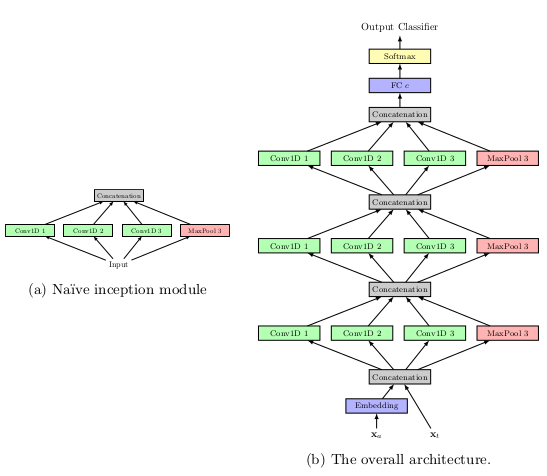
\includegraphics[width=15cm]{inception}
        \end{center}
        
        \medskip
        In ~\cite{10.1007/978-3-030-35166-3_25}, questa architettura 
        viene applicata al problema della Next Activity Prediction
        su dataset di Process Mining, mettendo a confronto
        l'approccio convoluzionale con metodi random e LSTM
        provandone la superiorit\`a sia in termini di accuratezza che 
        di tempo. 

        \newpage
        \section{Deformable Convolutions}
        \subsection{Introduzione}
        In ~\cite{DBLP:journals/corr/DaiQXLZHW17}, viene proposta una 
        soluzione al problema della gestione delle variazioni 
        geometriche nelle immagini, uno dei problemi chiave della 
        computer vision per il riconoscimento visivo. Gli approcci 
        classici prevedono tecniche di data augmentation sull'input, ad
        esempio applicando trasformazioni affini sugli esempi di
        training, o l'applicazione manuale di algoritmi e features 
        invarianti alle trasformazioni sviluppati in maniera diversa da
        caso a caso. Queste soluzioni classiche hanno tuttavia un paio
        di aspetti negativi. Nel primo caso le trasformazioni 
        geometriche sono assunte costanti e conosciute in modo da 
        migliorare i dati e progettare algoritmi ad hoc, ma ci\`o 
        impedisce di generalizzare su compiti con trasformazioni 
        diverse non propriamente modellate. Nel secondo caso, invece, 
        la progettazione di features e algoritmi invarianti alle 
        trasformazioni pu\`o essere molto difficile, nei casi in cui 
        queste trasformazioni, anche se conosciute, sono molto 
        complesse. In breve, una rete convoluzionale \`e per sua 
        natura limitata nella rappresentazione di grandi e sconosciute 
        trasformazioni. Ci\`o \`e dovuto alle strutture geometriche 
        fisse usate dalle CNN: un'unit\`a convoluzionale campiona la 
        feature map di input a posizioni fisse, un layer di pooling 
        riduce la risoluzione spaziale a un tasso predefinito, ecc.\\ 
        Sono assenti meccanismi interni per la gestione di 
        trasformazioni geometriche causando diversi problemi, come ad 
        esempio la dimensione costante del campo recettivo di tutte le 
        unit\`a d'attivazione in un layer, soluzione non auspicabile in 
        convoluzioni di alto livello che codificano il significato di 
        determinate posizioni spaziali. Diverse posizioni, infatti, 
        potrebbero corrispondere agli stessi oggetti a scala diversa o
        deformati; in un task di semantic segmentation per riconoscere 
        \textit{quali} oggetti si trovano all'interno di un'immagine, 
        sarebbe desiderabile essere in grado di adattare dinamicamente 
        diverse scale e le dimensioni del campo ricettivo.

        \subsection{Convoluzione Deformabile}
        La convoluzione 2-D consiste in due passaggi: campionamento su
        una tassellatura regolare $R$ della feature map di input e
        somma dei valori campionati pesati da $\boldsymbol{w}$.
        La tassellatura $R$, che ha la forma di una griglia, definisce
        il campo ricettivo della rete. Ad esempio
        \begin{equation} \label{eq:defconvgrid}
            R=\{(-1,-1), (-1,0),\dots,(0,1),(1,1)\}
        \end{equation}
        rappresenta un kernel $3\times 3$.

        \smallskip
        Nel dettaglio l'operazione di convoluzione \`e la seguente, per
        ogni $p_0$ nell'output $y$ pesato da $\boldsymbol{w}$:
        \begin{equation} \label{eq:defconv1}
            \boldsymbol{y}(\boldsymbol{p}_0) = 
            \sum\limits_{\boldsymbol{p}_n \in R} 
            \boldsymbol{w}(\boldsymbol{p}_n)\cdot 
            \boldsymbol{x}(\boldsymbol{p}_0+
            \boldsymbol{p}_n+\Delta \boldsymbol{p}_n)
        \end{equation}
        Dove $\boldsymbol{R}$ indica la tassellatura regolare di 
        campionamento, aumentata con gli offset \{$\Delta p_n \mid n = 
        1,\cdots,N$\} con $N=|R|$. Il campionamento avviene quindi sulle
        posizioni irregolari $p_n + \Delta p_n$, ma, essendo queste 
        tipicamente frazionali, l'equazione \ref{eq:defconv1} \`e implementata
        tramite interpolazione bilineare, diventando:
        \begin{equation} \label{eq:defconv2}
            \boldsymbol{x}(\boldsymbol{p})=\sum\limits_{\boldsymbol{q}}
            G(\boldsymbol{q},\boldsymbol{p})\cdot\boldsymbol{x}(\boldsymbol{q})
        \end{equation}
        dove $\boldsymbol{p}=\boldsymbol{p}_0+\boldsymbol{p}_n+
        \Delta\boldsymbol{p}_n$ indica un punto arbitrario frazionale, 
        $\textbf{q}$ enumera le posizioni in $\boldsymbol{x}$ e
        $G(\cdot,\cdot)$ \`e il kernel dell'interpolazione bilineare 
        definito come
        \begin{equation} \label{eq:defconv3}
            G(\boldsymbol{q}, \boldsymbol{p}) = g(q_x,p_x)\cdot 
            g(q_y,p_y)
        \end{equation}
        dove $g(a, b) = max(0, 1-\mid a-b\mid)$, che si 
        dimostra essere un'operazione di rapida esecuzione 
        essendo non nulla solo per poche $\boldsymbol{q}$. 
        ~\cite{DBLP:journals/corr/DaiQXLZHW17} 

        \subsection{Reti Deformabili}
        I moduli deformabili hanno lo stesso input e output delle loro
        controparti tradizionali, quindi non necessitano di modifiche
        per essere aggiunte ad un modello gi\`a esistente.
        Gli offset sono calcolati durante l'apprendimento tramite una
        apposito layer convoluzionale. L'apprendimento poi procede
        per retropropagazione tramite l'operazione di interpolazione
        bilineare delle equazioni \ref{eq:defconv2} e \ref{eq:defconv3}.
        In particolare, l'operazione di retropropagazione calcola il
        gradiente rispetto all'offset $\Delta\boldsymbol{p}_n$ tramite
        \begin{align} \label{eq:defconvbackprop}
            \frac{\partial\boldsymbol{y}(\boldsymbol{p}_0)}
            {\partial\Delta\boldsymbol{p}_n}&=
            \sum\limits_{\boldsymbol{p}_n\in{R}}
            \boldsymbol{w}(\boldsymbol{p}_n)\cdot
            \frac{\partial\boldsymbol{x}(\boldsymbol{p}_0+
            \boldsymbol{p}_n+\Delta\boldsymbol{p}_n)}
            {\partial\Delta\boldsymbol{p}_n}\\
            &=\sum\limits_{\boldsymbol{p}_n\in{R}}\left[
            \boldsymbol{w}(\boldsymbol{p}_n)\cdot
            \sum\limits_{\boldsymbol{q}}
            \frac{\partial G(\boldsymbol{q},\boldsymbol{p}_0+
            \boldsymbol{p}_n+\Delta\boldsymbol{p}_n)}
            {\partial\Delta\boldsymbol{p}_n}
            \boldsymbol{x}(\boldsymbol{q})\right]
        \end{align}
        dove $\frac{\partial G(\boldsymbol{q},\boldsymbol{p}_0+
        \boldsymbol{p}_n+\Delta\boldsymbol{p}_n)}
        {\partial\Delta\boldsymbol{p}_n}
        \boldsymbol{x}(\boldsymbol{q})$ deriva dall'equazione 
        \ref{eq:defconv3} e, essendo gli offset $\Delta\boldsymbol{p}_n$
        bidimensionali, $\partial\Delta\boldsymbol{p}_n$ viene usata per
        indicare $\partial\Delta\boldsymbol{p}_n^x$ e 
        $\partial\Delta\boldsymbol{p}_n^y$, per semplicit\`a.

    \chapter{Soluzione adottata}
    In questo lavoro di ricerca si \`e cercato di portare avanti il 
    lavoro iniziato da ~\cite{10.1007/978-3-030-35166-3_25} testando le
    performance di nuovi modelli convoluzionali rispetto ai classici
    approcci ricorrenti su dati 1-D e nello specifico del campo del
    process mining sviluppando una rete deformabile come in 
    ~\cite{DBLP:journals/corr/DaiQXLZHW17} adattata alla gestione di 
    dati sequenziali e una rete convoluzionale il cui kernel \`e 
    modificato da una maschera binaria costante. Mostreremo infine i 
    risultati confrontandoli con una rete convoluzionale standard.

    \section{Next-Activity Prediction}
    \subsection{Introduzione}
    Introduciamo alcuni concetti base di process mining per descrivere
    meglio il tipo di compito che le reti devono completare.
    In generale ogni tecnica di process mining punta ad estrarre
    informazioni utili da log di eventi di un processo aziendale,
    dove ogni evento fa riferimento a un'attivit\`a di un particolare
    caso, o traccia di processo.

    \smallskip
    Siano $\mathcal{A}$ l'insieme delle attivit\`a, $\mathcal{C}$ 
    l'insieme dei casi in termini dei loro identificatori e sia 
    $\mathcal{D}_i$ l'insieme degli attributi con $\forall 1\leq i\leq m$. 
    Un \textbf{evento} \`e una tupla $e=(a,c,t,d_1,\dots,d_m)$ dove 
    $a\in \mathcal{A}, c\in \mathcal{C}, t$ \`e il timestamp
    e $d_i\in \mathcal{D}_i$ sono eventuali altri attributi che non 
    verranno considerati nel continuo della descrizione, come in 
    ~\cite{10.1007/978-3-030-35166-3_25}. Dato un evento 
    $e=(a,c,t,d_1,\dots,d_m)$ \`e quindi possibile definire le funzioni
    $\pi_{\mathcal{A}}(e)=a,\pi_{\mathcal{C}}(e)=c,
    \pi_{\mathcal{T}}(e)=t$ e $\pi_{{\mathcal{D}}_i}(e)=d$.

    \smallskip
    Una \textbf{traccia} \`e una sequenza finita di eventi 
    $\sigma=\langle e_1, e_2, \dots, e_n\rangle$, con $e\in\mathcal{E}$ e
    $n=|\sigma|$, tale che $\pi_{\mathcal{T}}(e_i)\leq\pi_{\mathcal{T}}
    (e_{i+1})$ e $\pi_{\mathcal{C}}(e_i)\leq\pi_{\mathcal{C}}(e_{i+1}),
    \forall 1\leq i\leq n-1$. Data la traccia $\sigma=\langle
    e_1,e_2,\dots,e_n)$, un prefisso $\sigma^k$ di $\sigma$, con $k=|
    \sigma^k|\leq|\sigma|$, \`e la traccia $\sigma^k=\langle e_1,e_2,
    \dots,e_k\rangle$. In particolare, una traccia rappresenta un 
    processo completo, iniziato e completato, mentre un prefisso 
    rappresenta un processo in esecuzione (traccia corrente). Un 
    \textbf{event log}, infine, \`e un insieme di tracce tali per cui 
    ogni evento appare al pi\`u una volta in tutto il log.

    \subsection{Formulazione del compito}
    Il task di next-activity prediction consiste nella predizione
    dell'attivit\`a di un processo in esecuzione.
    Dato un log di eventi $\mathcal{L}=\{\sigma_i\}_{i=1}^N$ di $N$
    tracce, si costruisce un dataset 
    $\mathcal{S}=\{(s_i,a_i)\}_{i=1}^M$, con $M>N$, dove $s_i$ \`e una
    sequenza di eventi corrispondente al prefisso $\sigma_j^k$ di una
    traccia $\sigma_j\in\mathcal{L}$, con $k\in\mathbb{N}^+$, e 
    $a_i$ \`e l'attivit\`a del $(k+1)$-esimo evento della traccia
    $\sigma_j$. Formalmente, sia $\sigma=\langle e_1, e_2, \dots, e_n
    \rangle$ una traccia e $\Pi_{\mathcal{A}}(\sigma,k)=
    \pi_{\mathcal{A}}(e_k)$ la funzione che ritorna l'attivit\`a del 
    $k$-esimo evento di $\sigma$, allora
    \begin{equation}
        \mathcal{S}=\{(s_i,a_i)\}_{i=1}^M=
        \bigcup\limits_{j=1}^N\left\{
        (\sigma_j^{k_j},\Pi_{\mathcal{A}}(\sigma_j,k_j+1))
        \right\}_{k_j=1}^{|\sigma_j|}
    \end{equation}
    In particolare, $\mathcal{S}$ \`e il dataset di tutti i prefissi
    di tutte le tracce in $\mathcal{L}$ etichettate con l'attivit\`a
    successiva associata nella traccia corrispondente.

    \subsection{Rappresentazione delle Feature}
    Dato che $\mathcal{S}$ consiste di prefissi ed attivit\`a, \`e
    necessario convertire gli elementi di $\mathcal{S}$ in 
    rappresentazioni numeriche $\boldsymbol{x}\in\mathbb{R}^l$, con 
    $l\in\mathbb{N}^+$. Per ogni coppia $(s,a)=(\langle 
    e_1,e_2,\dots,e_k\rangle, a)\in\mathcal{S}$, costruiamo la
    corrispondente rappresentazione numerica $((\boldsymbol{x}_{act}, 
    \boldsymbol{x}_t),y)$. Sia $f:\mathcal{A}\rightarrow[1,2,\dots,
    \mathcal{C}]$ una funzione che assegna un valore numerico ad ogni
    attivit\`a, con $\mathcal{C}=|\mathcal{A}|$ \`e la cardinalit\`a
    del vocabolario delle attivit\`a, ad esempio il numero delle classi.
    Allora $\boldsymbol{x}_{act}=(x_1,x_2,\dots,x_k)$ \`e il vettore per
    il quale $x_i=f(\pi_A(e_i))\ \forall 1\leq i\leq k$, mentre 
    $\boldsymbol{x}_{t}=(x_1,x_2,\dots,x_k)$ \`e il vettore delle
    rappresentazioni numeriche delle informazioni temporali delle
    attivit\`a. Analogamente $y=f(a)$. 

    \newpage
    \section{Deformable ConvNet 1D} \label{sec:def}
    Dovendo gestire sequenze temporali anzich\`e immagini, \`e stato 
    necessario modificare l'equazione (\ref{eq:defconv3}) in modo
    da eseguire un'operazione di interpolazione lineare
    adeguata; verranno anche definiti in seguito i dettagli
    dell'implementazione.
    \subsubsection{Tassellatura regolare e offset}
    La tassellatura regolare che definisce il kernel 
    dell'operazione di convoluzione deformata \`e definita, 
    per dati sequenziali, come un vettore del tipo
    \begin{equation}
        R = (-k, \dots, -1, 0, 1, \dots, +k)
    \end{equation}
    con $k=\text{floor}(ks/2)$ e ks dimensione del kernel. 
    Per un kernel di dimensione 3 e strides=1, si avr\`a quindi
    \begin{equation}
        R = (-1, 0, 1)
    \end{equation}
    I valori dell'offset sono invece ottenuti tramite un layer
    convoluzionale tradizionale, calcolato con il doppio dei filtri 
    della feature map di input e same padding, sottratto all'input 
    stesso. Il risultato dell'operazione \`e poi sommato alla griglia
    regolare $\mathcal{R}$ per ottenere gli spostamenti degli indici di
    input che verranno calcolati tramite l'equazione 
    \begin{equation} \label{eq:5}
        G(\textbf{q}, \textbf{p}) = g(q, p)
    \end{equation}
    con g() invariata da $g(a, b) = max(0, 1-\mid a-b\mid)$.\\
    L'equazione completa \`e analoga all'equazione \ref{eq:defconv2}
    con il solo adattamento della funzione $G$ con quella dell'equazione
    precedente. Il risultato della convoluzione deformata \`e un tensore
    della stessa dimensione della feature map di input, quindi, da
    questo punto di vista, la convoluzione deformabile si comporta come
    una convoluzione standard con same padding. 

    \subsection{Implementazione}
    Il layer deformabile \`e stato implementato in Keras\footnote{https://keras.io}, 
    una libreria open-source di deep learning basata sul backend 
    TensorFlow\footnote{https://www.tensorflow.org/}, come una sottoclasse 
    di Layer, la superclasse che definisce un layer generico nella libreria.
    La classe padre \`e formata da tre metodi principali che ne definiscono il 
    comportamento. Il primo, \textbf{\_\_init\_\_()}, ha il compito di inizializzare 
    gli attributi della classe avendo come parametri di input il numero di filtri,
    la dimensione del kernel ed eventuali altri parametri come la funzione 
    d'attivazione o di regolarizzazione, il secondo, \textbf{build()}, definisce e 
    inizializza i pesi che verranno utilizzati nel layer e ha come parametro 
    la dimensione dell'input e il terzo, \textbf{call()}, contiene la logica del 
    layer avendo come parametro il tensore di input. 

    La sottoclasse DeformableConv1D implementa i tre metodi per override. 
    Il nuovo metodo \_\_init\_\_() inizializza gli attributi dei filtri e della 
    dimensione del kernel e definisce l'attributo della tassellatura regolare 
    \textbf{R} tramite il nostro metodo regularGrid(). Il metodo build(), invece, 
    crea il tensore dei pesi \textbf{W} della stessa dimensione del kernel. 
    Infine, il metodo call() genera il tensore degli offset dall'output di Conv1D,
    a sua volta sottoclasse di Layer e classe standard di Keras per layer 
    convoluzionali 1D, con padding 'same' e attivazione 'relu', per poi passarlo 
    come parametro insieme al tensore di input al nostro metodo linearInterpolation()
    che calcola i valori offsettati che vengono poi pesati dai parametri definiti 
    durante la fase di build() ottenendo l'output finale del layer.
    Lo pseudocodice dei metodi \`e riportato negli algoritmi \ref{alg:definit}, 
    \ref{alg:defbuild} e \ref{alg:defcall}, mentre il codice completo originale 
    \`e visibile nell'appendice \ref{code:def}.

    \begin{algorithm}[t] 
        \caption{Funzione \_\_init\_\_() di DeformableConv1D}
        \begin{algorithmic} \label{alg:definit}
            \REQUIRE Numero di filtri di output \textbf{f}, 
            Dimensione del kernel \textbf{ks}
            \STATE Inizializza gli attributi dei filtri e della dimensione del 
            kernel:\\ 
            \quad\textbf{filters} $\gets$ \textbf{f} \\
            \quad\textbf{kernel\_size} $\gets$ \textbf{ks} \\
            \STATE Inizializza l'attributo della tassellatura regolare R\\ 
            \quad\textbf{R} $\gets$ \textbf{regularGrid(kernel\_size)}
        \end{algorithmic}
    \end{algorithm}

    \begin{algorithm}[t]
        \caption{Funzione regularGrid}
        \begin{algorithmic} \label{alg:reggrid}
            \REQUIRE Dimensione del kernel \textbf{ks}
            \STATE Crea un array di interi della stessa dimensione del kernel 
            inizializzato a zero: \\\quad$\boldsymbol{R}\gets
            \text{zeros}(\boldsymbol{ks}, \text{int32})$
            \STATE Inizializza la variabile degli elementi della tassellatura:\\ 
            \quad$\boldsymbol{e}\gets-\text{floor}(\boldsymbol{ks}/2)$
            \FOR{i in range($\boldsymbol{ks}$)}
                \STATE Aggiorna l'elemento corrente della tassellatura:\\
                \quad$\boldsymbol{R}[i]\gets \boldsymbol{e}$
                \STATE Ottieni l'elemento successivo:\\
                \quad$\boldsymbol{e}\gets \boldsymbol{e}+1$
            \ENDFOR
            \RETURN R
        \end{algorithmic}
    \end{algorithm}

    \begin{algorithm}[t] 
        \caption{Funzione build() di DeformableConv1D}
        \begin{algorithmic} \label{alg:defbuild}
            \REQUIRE Dimensione dell'input \textbf{input\_shape},
            \STATE Inizializza la variabile della forma del tensore dei pesi:\\
            \quad W\_shape $\gets\text{shape}(\text{kernel\_size}, 1)$
            \STATE Dichiara il tensore dei pesi da apprendere e lo aggiunge alla 
            lista dei pesi associati al layer corrente:\\
            \quad$\boldsymbol{W}=\text{add\_weight}(\boldsymbol{W},
            \dots,trainable=True)$
        \end{algorithmic}
    \end{algorithm}

    \begin{algorithm}[t] 
        \caption{Funzione call() di DeformableConv1D}
        \begin{algorithmic} \label{alg:defcall}
            \REQUIRE Tensore di input $\boldsymbol{x}$,
            \STATE Definisci l'operazione di convoluzione 1D standard per il calcolo
            degli offset con 'same' padding:\\
            \quad\textbf{offconv}$\gets$\textbf{Conv1D}() dove Conv1D \`e il metodo 
            nativo di Keras di un layer convoluzionale 1D.
            \STATE Inizializza la variabile degli offset:\\
            \quad\textbf{offset}$\gets$\textbf{offconv}($\boldsymbol{x}$)
            \STATE Calcola il tensore delle locazioni interpolate:\\
            \quad $\boldsymbol{y}\gets\text{linearInterpolation}(\boldsymbol{x}, 
            \textbf{offset})$
            \STATE Pesa il tensore risultante con i pesi creati nel metodo build:\\
            \quad$\boldsymbol{y}\gets\sum_i\boldsymbol{W_i}*\boldsymbol{y}$
            \RETURN $\boldsymbol{y}$
        \end{algorithmic}
    \end{algorithm}

    \begin{algorithm}[t] 
        \caption{Funzione linearInterpolation() di DeformableConv1D}
        \begin{algorithmic} \label{alg:deflinint}
            \REQUIRE Tensore di input $\boldsymbol{x}$, 
            Tensore degli offset \textbf{offset}
            \STATE Definisci il tensore delle locazioni di input $\boldsymbol{Q}$
            \STATE Calcola il tensore delle distanze $\textbf{off}\gets
            \text{offset}-x$\\
            \quad\textbf{offset}$\gets$\textbf{offconv}($\boldsymbol{x}$)
            \STATE Calcola il tensore delle locazioni di input aumentate 
            dall'offset:\\
            \quad $\boldsymbol{P}\gets\boldsymbol{Q}-\boldsymbol{x}$ 
            \STATE Esegui l'operazione di interpolazione:\\
            \quad$\boldsymbol{y}=g(\boldsymbol{Q}, \boldsymbol{P}+\boldsymbol{R})$
            \RETURN $\boldsymbol{y}$
        \end{algorithmic}
    \end{algorithm}

    \begin{algorithm}[t] 
        \caption{Funzione g() di DeformableConv1D}
        \begin{algorithmic} \label{alg:defg}
            \REQUIRE Tensore $\boldsymbol{q}$, Tensore $\boldsymbol{p}$
            \STATE Esegui l'operazione di interpolazione lineare 
            $G\gets\max(0, 1-|q-p|)$
            \RETURN $G$
        \end{algorithmic}
    \end{algorithm}

    \section{Masked ConvNet} \label{sec:mask}
    Si \`e voluto implementare contemporaneamente, un layer 
    convoluzionale standard dal kernel costante. In particolare viene 
    applicata una maschera binaria casuale, generata in fase di 
    pretraining. L'effetto della maschera \`e quello di generare un 
    tensore sparso che deforma il kernel che ignora conseguentemente 
    alcuni valori del campo ricettivo che rappresenta. 
    La maschera, cos\`i come il kernel stesso, non \`e considerata come
    un parametro da apprendere, ma rimane costante una volta definita 
    per un certo layer riducendo il numero di parametri totali appresi
    dalla rete.

    \subsection{Implementazione}
    Il layer a kernel fisso MaskedConv1D \`e implementato come sottoclasse di Conv1D
    della quale implementa per override solo due metodi. Il metodo \_\_init\_\_() 
    chiama il costruttore della superclasse specificando di non apprendere i pesi
    del layer corrente, mentre il metodo call() genera la maschera binaria e la 
    applica al kernel generato dal metodo build(), che viene sempre chiamato subito
    prima dell'esecuzione del corpo del metodo call(). Lo pseudocodice del metodo
    call() \`e definito nell'algoritmo \ref{alg:maskcall} mentre il codice completo
    \`e presente nell'appendice \ref{code:mask}.

    \begin{algorithm}[t] 
        \caption{Funzione call() di MaskedConv1D}
        \begin{algorithmic} \label{alg:maskcall}
            \REQUIRE Tensore di input $\boldsymbol{x}$
            \STATE Genera la maschera binaria delle stesse dimensioni del kernel:\\
            \quad \textbf{mask}$\gets \text{rand}(2, 
            \text{size}=(\text{kernel\_size}, 1, 1))$
            \STATE Dove rand \`e una funzione che genera valori interi casuali e il 
            cui primo parametro definisce il range di valori da generare, partendo da
            zero, mentre il secondo ne definisce la dimensionalit\`a.
            \STATE Aggiorna il kernel applicandovi la maschera binaria:\\
            $\text{kernel}\gets\text{kernel}*\text{mask}$
            \STATE Chiama il metodo della superclasse per completare la convoluzione:
            \\\quad$super.call()$
        \end{algorithmic}
    \end{algorithm}

    \section{Dettagli Architetturali}
    Dato il dataset di training $\mathcal{D}=\{(x_{act}^i,x_t^i),y^i\}_{i=1^M}$, 
    l'input delle architetture \`e dato dalla concatenazione del risultato di un 
    \textit{embedding} layer, che associa ogni parola di $x_{act}$ in un vettore 
    di dimensione fissa in $\mathbb{R}^d$ con $d=\text{ceil}(C/2)$, con
    l'input temporale $x_t$ di valori in $\mathbb{R}^{k\times d}$ per
    una rappresentazione finale di valori in $\mathbb{R}^{k\times d+1}$.

    Si susseguono poi una serie di layer convoluzionali e di max pooling
    il cui ultimo layer \`e input di un layer Dense il cui output \`e
    usato per calcolare le probabilit\`a finali tramite una attivazione
    softmax (sezione \ref{sec:softmax}). Come non linearit\`a degli 
    hidden layer si \`e scelto di usare una attivazione ReLU (sezione
    \ref{sec:activation}).

    Per testare le performance dei nuovi modelli, si sono valutate tre
    reti per ogni approccio (standard, deformabile e costante) 
    differenti solo nel numero di moduli convoluzionali in sequenza tra
    loro. In particolare sono state implementate reti da uno, due e tre
    moduli successivi, in cui ogni layer, ove possibile, aveva un kernel
    (o una griglia regolare per le convoluzioni deformabili) di 
    lunghezza 3, seguito da un layer di max pooling.

    \section{Software e Hardware utilizzati}
    La performance dei modelli \`e stata testata sui seguenti cinque 
    diversi dataset di process mining, come in 
    ~\cite{10.1007/978-3-030-35166-3_25}, e per ognuno di essi, si \`e 
    effettuata una 3-fold cross validation (sezione \ref{sec:crossval}).
    Le metriche utilizzate sono il punteggio Brier e la accuracy. Il 
    punteggio Brier pu\`o essere interpretato come una misura della 
    calibrazione di un insieme di predizioni, calcolando l'errore 
    quadratico medio della previsione per un certo elemento dell'input 
    con il valore reale, ripetendo per ogni elemento dell'input. Il
    punteggio di Brier, quindi, \`e tanto migliore quanto pi\`u \`e 
    \textbf{basso}. I log adottati, le cui statistiche sono riportate nella tabella
    \ref{table:dataset}, sono i seguenti:
    \begin{itemize}
        \item[-] Receipt phase\footnote{https://doi.org/10.4121/uuid:a07386a5-7be3-4367-9535-70bc9e77dbe6}: contiene i record dell'esecuzione
            della fase di ricevuta del processo di applicazione
            del permesso di costruzione in un anonimo comune olandese.
        \item[-] helpdesk
            \footnote{https://doi.org/10.17632/39bp3vv62t.1}: 
            contiene gli eventi di un processo di biglietteria del 
            reparto helpdesk di una software agency italiana.
        \item[-] sepsis\footnote{https://doi.org/10.4121/uuid:915d2bfb-7e84-49ad-a286-dc35f063a460}: 
            contiene eventi di casi di sepsi registrati dal sistema ERP
            di un ospedale.
          \item[-] bpi12\footnote{https://doi.org/10.4121/uuid:3926db30-f712-4394-aebc-75976070e91f}:
            descrive il processo di un'applicazione di prestiti. 
            Preprocessato come in \cite{pred-bpm-lstm}.
          \item[-] nasa\footnote{https://doi.org/10.4121/uuid:60383406-ffcd-441f-aa5e-4ec763426b76}:
            contiene eventi al livello di chiamate dei metodi della
            classe NASA Crew Exploration Vehicle descritti da una
            esecuzione di una esaustiva suite di test d'unit\`a.
    \end{itemize}
    \begin{table}[t]
    \caption{Statistiche dei dataset}
    \begin{center} \label{table:dataset}
    \begin{tabular}[t]{llll}
        \hline
                        & classi    & casi  & sequenze \\
        Receipt phase   & 26        & 1434  & 7143     \\
        helpdesk        & 8         & 3804  & 9906     \\
        sepsis          & 16        & 1050  & 14164    \\
        nasa            & 47        & 2566  & 71072    \\
        bpi12           & 22        & 13087 & 151419   \\
        \hline
    \end{tabular}
    \end{center}
    \end{table}
    L'addestramento delle reti sfrutta la libreria di hyperparameter
    optimization "hyperopt"
    \footnote{https://github.com/hyperopt/hyperopt} per la scelta della
    combinazione migliore degli iperparametri della rete utilizzando
    il 20\% del training set come validation set scegliendo la 
    configurazione di parametri con il valore di loss in validazione
    migliore. Come in ~\cite{10.1007/978-3-030-35166-3_25}, l'algoritmo 
    di ottimizzazione per la scelta degli iperparametri \`e un 
    Parzen Estimator ad albero. L'ottimizzazione dei pesi, si basa
    sull'algoritmo Adam (sezione \ref{adam}), mentre si \`e optato per
    una regolarizzazione tramite early stopping (sezione 
    \ref{sec:regularization}), fermando la fase di training dopo aver
    smesso di osservare miglioramenti nella loss per 20 epoche 
    consecutive su un limite di 200 epoche massime.

    Si \`e scelto di implementare i layer definiti precedentemente in 
    Python3 tramite la libreria Keras\footnote{https://keras.io} usando
    il backend Tensorflow 2.0\footnote{https://www.tensorflow.org}. 
    L'addestramento delle reti \`e avvenuto sulla piattaforma online 
    fornita da Google Colab in contemporanea a una macchina locale per 
    lo sviluppo. I tempi d'esecuzione sono riportati nelle tabelle
    \ref{table:time1}, \ref{table:time2} e \ref{table:time3}.

    \begin{table}[t]
    \caption{Numero di parametri e tempo d'apprendimento in secondi 
        dalla media delle tre fold su tutti i log per le architetture
        a un solo modulo.}
    \begin{center}  \label{table:time1}
    \begin{tabular}{lrrrcrrr}
    & \multicolumn{3}{c}{\# parametri} & & \multicolumn{3}{c}{tempo(s)} \\
    & Std & Def & Mask & & Std & Def & Mask \\
    \cline{2-4} \cline{6-8}
    receipt     & 1716 & 1975 & 1268 &  &  27.8 &  43.2 &  65.4 \\ 
    helpdesk    &  821 &  256 &  341 &  &  11.6 &  15.8 &  23.4 \\
    sepsis      & 1456 &  675 &  688 &  &  20.6 &  55.2 &  31.4 \\ 
    nasa        & 5015 & 5810 & 2711 &  & 131.9 & 239.2 &  96.2 \\ 
    bpi12       & 2186 & 1453 & 1034 &  & 196.1 & 376.5 & 205.9 \\ 
    \end{tabular}
    \end{center}
    \end{table}
    
    \begin{table}[t]
    \caption{Numero di parametri e tempo d'apprendimento in secondi 
        dalla media delle tre fold su tutti i log per le architetture
        a due moduli.}
    \begin{center} \label{table:time2}
    \begin{tabular}{lrrrcrrr}
    \hline
    & \multicolumn{3}{c}{\# parametri} & & \multicolumn{3}{c}{tempo(s)} \\
    & Std & Def & Mask & & Std & Def & Mask \\
    \cline{2-4} \cline{6-8}
    receipt     & 5716 & 3182 & 1300 &  &  13.9 &  55.2 &  41.3 \\
    helpdesk    & 3925 &  419 &  373 &  &  16.9 &  21.7 &  49.1 \\
    sepsis      & 4560 & 1078 &  720 &  &  70.9 &  82.6 &  39.8 \\ 
    nasa        & 8119 & 9317 & 2743 &  & 118.5 & 336.7 & 119.0 \\ 
    bpi12       & 5290 & 2344 & 1066 &  & 222.5 & 205.2 & 272.2 \\ 
    \hline
    \end{tabular}
    \end{center}
    \end{table}
    
    \begin{table}[t]
    \caption{Numero di parametri e tempo d'apprendimento in secondi 
        dalla media delle tre fold su tutti i log per le architetture
        a tre moduli.}
    \begin{center} \label{table:time3}
    \begin{tabular}{l rrrcrrr}
    \hline
    & \multicolumn{3}{c}{\# parametri} & & \multicolumn{3}{c}{tempo(s)} \\
    & Std & Def & Mask & & Std & Def & Mask \\
    \cline{2-4} \cline{6-8}
    receipt     &  8820 &  4389 & 1332 & &  99.6 &  49.7 & 140.2 \\
    helpdesk    &  7029 &   582 &  405 & &  41.3 &  26.4 & 101.1 \\
    sepsis      &  7664 &  1481 &  752 & &  52.6 & 139.9 &  94.0 \\ 
    nasa        & 11223 & 12824 & 2775 & & 229.6 & 219.2 & 133.7 \\ 
    bpi12       &  8394 &  3235 & 1098 & & 188.2 & 217.7 & 420.9 \\ 
    \hline
    \end{tabular}
    \end{center}
    \end{table}

    \newpage
    \section{Conclusioni}
    \subsection{Risultati a confronto}
    Le tabelle \ref{table:time1}, \ref{table:time2} e \ref{table:time3}
    mostrano come il numero di parametri delle soluzioni implementate
    sia quasi sempre minore di quello delle convoluzioni standard,
    indicando le minori dimensioni dei modelli proposti.
    In termini di metriche, visibili nelle tabelle \ref{table:results1}, 
    \ref{table:results2} e \ref{table:results3} l'approccio deformabile 
    ha mostrato, su una media dei tre test effettuati, una accuracy e un brier 
    score marginalmente migliori concorrendo a validare l'ipotesi di partenza che le
    variazioni nei valori temporali di un processo possano essere paragonabili alle 
    variazioni geometriche in un'immagine e affrontate con gli stessi mezzi
    nonch\`e l'importanza del ruolo del campo ricettivo di una rete convoluzionale.

    \begin{table}[t]
    \caption{Risultati delle tre convoluzioni testate nelle architetture 
        a singolo modulo. I risultati sono stati calcolati effettuando 
        la media delle tre iterazioni del 3-fold cross validation e la 
        relativa deviazione standard.}
    \begin{center} \label{table:results1}
    \begin{tabular}{llcc}
    \hline
    \multicolumn{4}{c}{\textbf{Modulo Singolo}} \\
    \hline
    \textbf{dataset} & \textbf{metodo} & \textbf{brier score} & \textbf{accuracy} \\
    \hline
    helpdesk & standard    & 0.044 $\pm$ 0.001 & 0.775 $\pm$ 0.007 \\
    helpdesk & deformable  & 0.043 $\pm$ 0.001 & 0.774 $\pm$ 0.005 \\
    helpdesk & masked      & 0.044 $\pm$ 0.001 & 0.768 $\pm$ 0.006 \\
    \hline
    receipts & standard    & 0.011 $\pm$ 0.000 & 0.813 $\pm$ 0.003 \\
    receipts & deformable  & 0.009 $\pm$ 0.000 & 0.860 $\pm$ 0.001 \\
    receipts & masked      & 0.010 $\pm$ 0.000 & 0.829 $\pm$ 0.004 \\
    \hline
    sepsis   & standard    & 0.030 $\pm$ 0.001 & 0.627 $\pm$ 0.018 \\
    sepsis   & deformable  & 0.031 $\pm$ 0.000 & 0.633 $\pm$ 0.005 \\
    sepsis   & masked      & 0.034 $\pm$ 0.001 & 0.552 $\pm$ 0.007 \\
    \hline
    nasa     & standard    & 0.003 $\pm$ 0.000 & 0.891 $\pm$ 0.002 \\
    nasa     & deformable  & 0.003 $\pm$ 0.000 & 0.891 $\pm$ 0.002 \\
    nasa     & masked      & 0.005 $\pm$ 0.000 & 0.821 $\pm$ 0.010 \\
    \hline
    bpi12    & standard    & 0.014 $\pm$ 0.000 & 0.774 $\pm$ 0.000 \\
    bpi12    & deformable  & 0.014 $\pm$ 0.000 & 0.768 $\pm$ 0.004 \\
    bpi12    & masked      & 0.017 $\pm$ 0.000 & 0.729 $\pm$ 0.004 \\
    \hline
    media    & standard    & 0.0204 & 0.776 \\
    media    & deformable  & 0.0200 & 0.785 \\
    media    & masked      & 0.0220 & 0.740 \\
    \hline
    \end{tabular}
    \end{center}
    \end{table}

    \begin{table}[t]
    \caption{Risultati delle tre convoluzioni testate nelle architetture
        a due moduli. I risultati sono stati calcolati effettuando 
        la media delle tre iterazioni del 3-fold cross validation e la 
        relativa deviazione standard.}
    \begin{center} \label{table:results2}
    \begin{tabular}{llcc}
    \hline
    \multicolumn{4}{c}{\textbf{Modulo Doppio}} \\
    \hline
    \textbf{dataset} & \textbf{metodo} & \textbf{brier score} & \textbf{accuracy} \\
    \hline
    helpdesk & standard    & 0.044 $\pm$ 0.001 & 0.774 $\pm$ 0.004 \\
    helpdesk & deformable  & 0.043 $\pm$ 0.001 & 0.774 $\pm$ 0.006 \\
    helpdesk & masked      & 0.044 $\pm$ 0.001 & 0.769 $\pm$ 0.005 \\
    \hline
    receipts & standard    & 0.010 $\pm$ 0.000 & 0.838 $\pm$ 0.002 \\
    receipts & deformable  & 0.009 $\pm$ 0.000 & 0.863 $\pm$ 0.005 \\
    receipts & masked      & 0.010 $\pm$ 0.000 & 0.829 $\pm$ 0.002 \\
    \hline
    sepsis   & standard    & 0.031 $\pm$ 0.000 & 0.628 $\pm$ 0.009 \\
    sepsis   & deformable  & 0.032 $\pm$ 0.000 & 0.615 $\pm$ 0.007 \\
    sepsis   & masked      & 0.035 $\pm$ 0.002 & 0.571 $\pm$ 0.030 \\
    \hline
    nasa     & standard    & 0.003 $\pm$ 0.000 & 0.887 $\pm$ 0.003 \\
    nasa     & deformable  & 0.003 $\pm$ 0.000 & 0.893 $\pm$ 0.002 \\
    nasa     & masked      & 0.003 $\pm$ 0.000 & 0.865 $\pm$ 0.011 \\
    \hline
    bpi12    & standard    & 0.014 $\pm$ 0.000 & 0.773 $\pm$ 0.001 \\
    bpi12    & deformable  & 0.014 $\pm$ 0.000 & 0.773 $\pm$ 0.001 \\
    bpi12    & masked      & 0.015 $\pm$ 0.000 & 0.755 $\pm$ 0.006 \\
    \hline
    media    & standard    & 0.0204 & 0.780 \\
    media    & deformable  & 0.0202 & 0.777 \\
    media    & masked      & 0.0214 & 0.765 \\
    \hline
    \end{tabular}
    \end{center}
    \end{table}

    \begin{table}[t]
    \caption{Risultati delle tre convoluzioni testate nelle architetture
        a tre moduli. I risultati sono stati calcolati effettuando 
        la media delle tre iterazioni del 3-fold cross validation e la 
        relativa deviazione standard.}
    \begin{center} \label{table:results3}
    \begin{tabular}{llcc}
    \hline
    \multicolumn{4}{c}{\textbf{Modulo Triplo}} \\
    \hline
    \textbf{dataset} & \textbf{metodo} & \textbf{brier score} & \textbf{accuracy} \\
    \hline
    helpdesk & standard    & 0.044 $\pm$ 0.001 & 0.773 $\pm$ 0.005 \\
    helpdesk & deformable  & 0.043 $\pm$ 0.000 & 0.773 $\pm$ 0.004 \\
    helpdesk & masked      & 0.045 $\pm$ 0.001 & 0.765 $\pm$ 0.011 \\
    \hline
    receipts & standard    & 0.010 $\pm$ 0.000 & 0.841 $\pm$ 0.002 \\
    receipts & deformable  & 0.009 $\pm$ 0.000 & 0.860 $\pm$ 0.006 \\
    receipts & masked      & 0.011 $\pm$ 0.000 & 0.822 $\pm$ 0.007 \\
    \hline
    sepsis   & standard    & 0.030 $\pm$ 0.000 & 0.639 $\pm$ 0.001 \\
    sepsis   & deformable  & 0.031 $\pm$ 0.001 & 0.632 $\pm$ 0.005 \\
    sepsis   & masked      & 0.036 $\pm$ 0.001 & 0.554 $\pm$ 0.006 \\
    \hline
    nasa     & standard    & 0.003 $\pm$ 0.000 & 0.890 $\pm$ 0.004 \\
    nasa     & deformable  & 0.003 $\pm$ 0.000 & 0.892 $\pm$ 0.003 \\
    nasa     & masked      & 0.004 $\pm$ 0.001 & 0.831 $\pm$ 0.040 \\
    \hline
    bpi12    & standard    & 0.014 $\pm$ 0.000 & 0.774 $\pm$ 0.001 \\
    bpi12    & deformable  & 0.014 $\pm$ 0.000 & 0.774 $\pm$ 0.000 \\
    bpi12    & masked      & 0.016 $\pm$ 0.000 & 0.745 $\pm$ 0.002 \\
    \hline
    media    & standard    & 0.0202 & 0.783 \\
    media    & deformable  & 0.0204 & 0.779 \\
    media    & masked      & 0.0220 & 0.751 \\
    \hline
    \end{tabular}
    \end{center}
    \end{table}

    \subsection{Sviluppi Futuri}
    Sono da indagare i contributi di ogni punto nel campo ricettivo deformato e da 
    testare diverse forme di inizializzazione dei pesi che possono influenzare 
    differentemente la struttura del campionamento seguendo le intuizioni di alcuni 
    recenti studi~\cite{luo2017understanding} sulle caratteristiche del campo 
    ricettivo delle reti convoluzionali, che gi\`a preannunciavano la validit\`a 
    teorica di un approccio deformabile, ed ampliando l'area di ricerca nelle
    reti convoluzionali in contesti diversi dalla computer vision. 

    \subsection{Riepilogo}
    In questo lavoro di tesi, si sono proposte due soluzioni convoluzionali
    per la soluzione della predizione dell'attivit\`a successiva di una
    traccia in esecuzione, uno dei pi\`u complessi compiti di process mining.
    A confronto con una rete convoluzionale tradizionale, l'approccio deformabile
    si \`e mostrato pi\`u performante su diversi dataset tratti da log reali, 
    provando la validit\`a del lavoro effettuato.

    \appendix
    \chapter{Codice}
    \section{DeformableConv1D} \label{code:def}
    \begin{lstlisting}[language=Python]
    import tensorflow as tf
    import tensorflow.keras.backend as K
    from tensorflow.keras.layers import Layer, Conv1D, Dense
    from tensorflow.python.keras.utils import conv_utils
    from tensorflow.python.framework import tensor_shape
    from tensorflow.python.ops import nn_ops
    import numpy as np
    
    # Deformable 1D Convolution
    class DeformableConv1D(Layer):
        def __init__(self, filters, kernel_size=3):
            super(DeformableConv1D, self).__init__()
            self.filters = filters
            self.kernel_size = kernel_size
            self.R = tf.constant(self.regularGrid(self.kernel_size), 
                                                  tf.float32)
        def build(self, input_shape):
            W_shape = (self.kernel_size, 1)
            self.W = self.add_weight(
                name='W',
                shape=W_shape,
                trainable=True,
                dtype=self.dtype)
            super(DeformableConv1D, self).build(input_shape)
    
        def call(self, x):
            offconv = Conv1D(x.shape[-1]*2, self.kernel_size, 
                             padding='same', activation='relu', 
                             trainable=True)
            offset = offconv(x)
            y = self.linearInterpolation(x, offset)
            y = tf.reduce_sum(self.W * y, [0])
            y = tf.reshape(y, [-1, x.shape[1], x.shape[2]])
            return y
    
        """
           Regular grid
           kernel_size: integer
        """
        def regularGrid(self, kernel_size):
            R = np.zeros(kernel_size, dtype='int32')
            j = -(np.floor(kernel_size/2))
            for i in range(R.shape[0]):
                R[i] = j
                j += 1
            return R
    
        """
            linear interpolation
            x: (b, ts, c)
            offset: (b, ts, c)
        """
        def linearInterpolation(self, x, offset):
            # input locations
            Q = tf.where(tf.equal(K.flatten(x), K.flatten(x)))
            Q = tf.cast(Q, tf.float32)
    
            offset = offset - x
            offset = K.flatten(offset)
    
            # offset locations
            P = Q + offset
    
            # regulard grid sampling
            # unstack necessary to bypass colab memory cap
            ylist = []
            for pn in tf.unstack(self.R):
              G = self.g(Q, P+pn)
              ylist.append(G * K.flatten(x))
    
            return tf.stack(ylist)
    
        """
            linear interpolation kernel
            q: input location
            p: offset location
        """
        def g(self, q, p):
            g = tf.subtract(tf.squeeze(q), tf.squeeze(p))
            g = tf.abs(g)
            g = tf.subtract(1.0, g)
            return tf.maximum(0.0, g)
        \end{lstlisting}
    
        \section{MaskedConv1D} \label{code:mask}
        \begin{lstlisting}[language=Python]
        import tensorflow as tf
        from tensorflow.keras.layers import Conv1D
        from numpy import random.randint as rand
        
        # Masked 1D Convolution
        class MaskedConv1D(Conv1D):
            def __init__(self, filters, kernel_size, **kwargs):
                super(MaskedConv1D, self).__init__(filters, 
                                                   kernel_size, 
                                                   trainable=False,
                                                   **kwargs)
        
            def call(self, x):
                # random boolean mask
                mask = rand(2, size=(self.kernel_size[0],1, 1))
                self.kernel = self.kernel * mask
                return super(MaskedConv1D, self).call(x)
        \end{lstlisting}
\bibliographystyle{ieeetr}
\bibliography{articoli}
\end{document}
